\documentclass[letterpaper]{article}
\usepackage{amsmath}
\usepackage{amsfonts}
\usepackage{fontspec}
\usepackage{graphicx}
\usepackage{float}		%\begin{figure}[H] <- agrega el H
\usepackage{multirow}
\usepackage{multicol}
\usepackage{indentfirst}
\usepackage{caption} %comando \ContinuedFloat
\usepackage{array} %paquete para tabular
\usepackage{subcaption} %subfiguras y continuación de figura
\usepackage{pstricks-add}
\usepackage{bm}
\usepackage{enumitem} %cara utilizar distintos enumerate item
\usepackage{listings} %para poner codigos


\newcolumntype{P}[1]{>{\centering\arraybackslash}p{#1}} % P{} (mayúscula) en vez de p{} (minúscula)
\newcommand{\vect}[1]{\boldsymbol{#1}} %notación vector \vect{•}
\renewcommand{\contentsname}{Índice}
\renewcommand{\figurename}{Figura}
\renewcommand{\tablename}{Tabla}
\renewcommand\refname{Referencias}

%%% quita los ":" del \caption
\makeatletter
\long\def\@makecaption#1#2{%
\vskip\abovecaptionskip
\sbox\@tempboxa{#1. #2}%
\ifdim \wd\@tempboxa >\hsize
#1. #2\par
\else
\global \@minipagefalse
\hb@xt@\hsize{\hfil\box\@tempboxa\hfil}%
\fi
\vskip\belowcaptionskip}
\makeatother
%%%%%%%%%%%%%%%%%%%%%%%%%


\pagestyle{plain}


%FORMATO PÁGINA
%\hoffset
\voffset=-2cm
\oddsidemargin=0.8cm
%\evensidemargin
%\topmargin 		%entre sup y encab
%\headheight		%tamaño encabezado
%\headsep			%sep encab y text
\textheight=23cm		%altura texto
\textwidth=15cm		%ancho texto
%\marginparsep	%sep notmargen y text
%\marginparwidth	%ancho nota al marg
\footskip=1cm		%pie de pag

\begin{document}

\thispagestyle{empty}

\hspace{-5mm}
\begin{minipage}[c]{7cm}
\centering

\includegraphics[width=4cm]{logoutfsm.jpg} \\
Universidad Técnica Federico Santa María
\end{minipage}
\hfill
\hspace{20mm}
\begin{minipage}[c]{7cm}
\centering

\includegraphics[width=4cm]{logomec1.jpg} \\
Departamento de Ingenieria Mecánica
\end{minipage}

\begin{center}
\vfill
 \Huge{{\bf Proyecto 1 }} \\ \vspace{1cm} 
 \Huge{Dinámica de fluidos computacional}
\vfill
\end{center}

\vfill \hfill
\begin{tabular}{l @{ : } l}
Nombre &   Ignacio Apablaza \\
Rol & 201141007-6  \\
Profesores & Romain Gers \\
			& Olivier Skurtys \\
Asignatura & IPM468 \\
\end{tabular}

\newpage
%---------------------------------------------


\tableofcontents


\newpage
%---------------------------------------------

\section{Introducción}

En el presente trabajo se estudia el método de diferencias finitas aplicado a la resolución de problemas modelados por ecuaciones diferenciales. El estudio se basa en programar distintas rutinas escritas en lenguaje Fortran que permite implementar los algoritmos a estudiar. Se divide en en tres secciones: La primera parte  consiste en el estudio del parámetro \texttt{precision} que permite establecer el número de cifras significativas asociada a un objeto de programación, y cómo la elección de este parámetro afecta los cálculos numéricos. \\

La segunda parte se estudia el comportamiento de una arteria sometida a esfuerzos asociados al bombeo sanguineo. Se modela el radio de la pared de la arteria como cilindros que se deforman radialmente y dicho comportamiento puede modelarse como una ecuación diferencial lineal de primer orden o como una ecuación diferencial hiperbólica, dependiendo de los supuestos escogidos. Se implementan los métodos de integración temporal Euler Implícito, Crank Nicolson, Leap-Frog y Newmark. La idea es estudiar la estabilidad del método teóricamente y comparar los resultados obtenidos por el programa implementado.\\

La última parte está orientada a la implementación al estudio de la resolución de sistemas dinámicos caóticos, correspondientes a modelos simplificados de la convección de Rayleight-Benand. Se obtiene un sistema de ecuaciones diferenciales de orden 1, tridimensional y no lineal. Se implementan una rutina Runge Kutta 4 (RK4) para la resolución del sistema. Se estudia además el comportamiento del mismo al variar los parametros que lo gobiernan.\\

Se anexa al final del informe los cógidos y rutina implementadas.




\newpage
%---------------------------------------------

\section{Metodología}
Ecuación de onda

\begin{equation}
\dfrac{\partial^2 y}{\partial t^2} - \gamma \dfrac{\partial^2 y}{\partial x^2} = f
\end{equation} 

Esquema de discretización Newmark

\begin{equation}
v = \dfrac{\partial u}{\partial t}
\end{equation}

Luego, el desarrollo de Taylor de $v(t+ \Delta t) = t^{n+1}$ para un paso de tiempo $\Delta t$ es

\begin{equation}
v^{n+1} = v^{n} + \Delta t \dfrac{\partial v}{\partial t} (t= \xi)
\end{equation}

para $\xi \in [t,t+\Delta t]$ .como

\begin{equation}
\dfrac{\partial v}{partial t} = \dfrac{\partial^2 u}{\partial t^2} = \gamma \dfrac{\partial^2 u}{\partial x^2} + f 
\end{equation}

Reemplazando en la (ECUACION!) se tiene 

\newpage
%---------------------------------------------

\section{Desarrollo y Análisis} \label{DESARROLLO_Y_ANALISIS}

%----

\subsection{Ejercicios en Fortran}
\subsubsection{Ejercicio 1}

Sea $A(n)$ un número real tal que
\begin{equation}
A(n) = \sum_{n=1}^\infty \dfrac{1}{n}
\end{equation}
Se implementa una programa en Fortran que permite calcular y graficar $A(n)$ para ciertos valores de $n$. En la Figura \ref{fig_P1_1_1} se grafica $A$ para simple y doble precisión. En la Figura \ref{fig_P1_1_2} Para doble y cuadruple precisión

\begin{figure} [H]
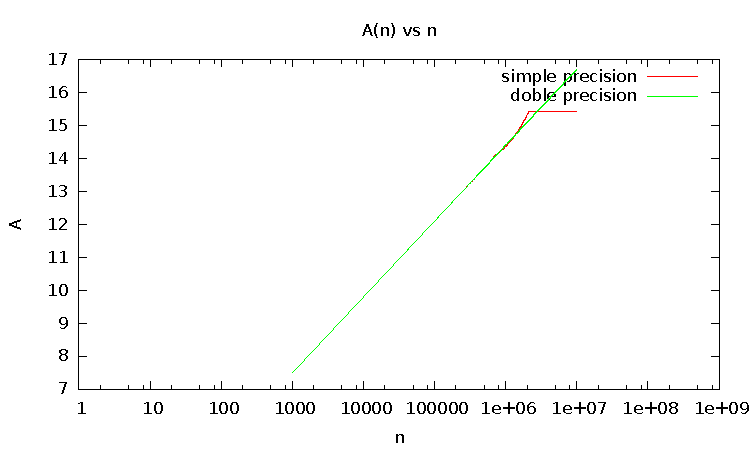
\includegraphics{./parte2/graficos/grafico_p1_1.pdf}
\caption{} \label{fig_P1_1_1}
\end{figure}

\begin{figure} [H]
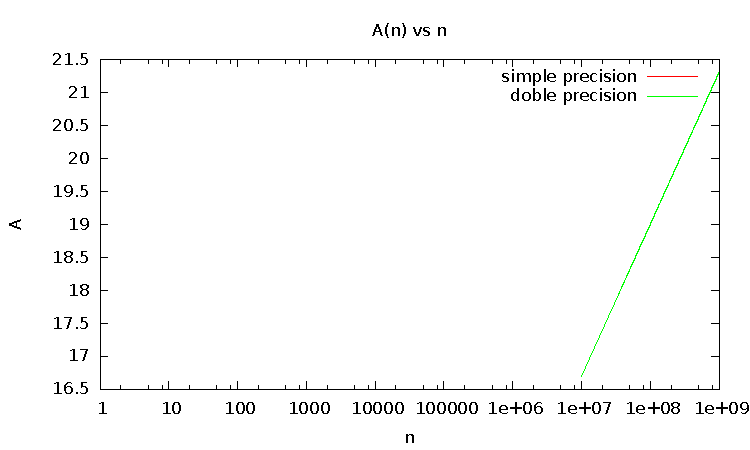
\includegraphics{./parte2/graficos/grafico_p1_2.pdf}
\caption{} \label{fig_P1_1_2}
\end{figure}

%----------------------------------------------
\subsubsection{Ejercicio 2}
Se implementa una rutina en Fortran que permite calcular los $n+1$ valores de la serie Fibonacci
\begin{equation}
u_{n+1} = u_{n} + u_{n-1} \hspace{1cm} \mbox{tal que} \hspace{0,5cm} u_0=0 \hspace{0,1cm} ; \hspace{0,1cm} u_1=1
\end{equation}
La serie se grafica para $n=100$

\begin{figure} [H]
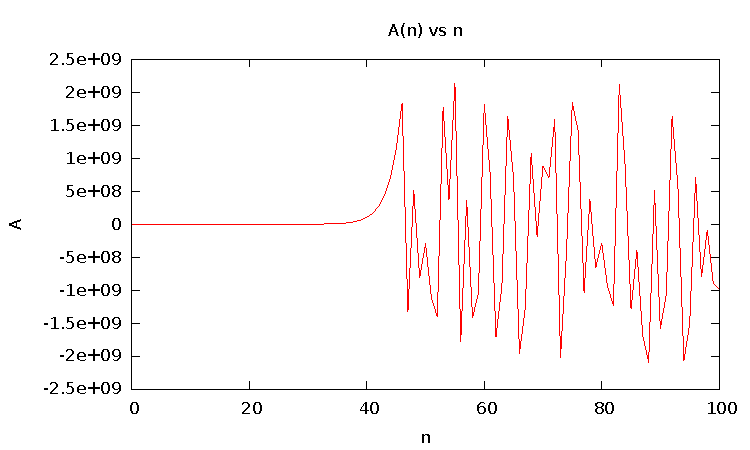
\includegraphics{./parte2/graficos/grafico_p2.pdf}
\caption{} \label{fig_P1_2}
\end{figure}

%----

\subsection{Estudio del comportamiento mecánico de una arteria}
%Estudio del comportamiento mecánico de una arteria

\subsection{Parte 1: Movimiento de una pared arterial}

Una arteria puede modelarse por un cilindro flexible de base circular, longitud $L$, radio $R_0$, cuyas paredes poseen un espesor $H$. Se supone que está constituido de un material elástico, incompresible, homogéneo e isotrópico. \\

Un modelo simplificado que describe el comportamiento mecánico de la pared arterial en interacción con el flujo sanguíneo se obtiene considerando que el cilindro es constituido por un conjunto de anillos independientes uno de otros. De esta manera se puede despreciar las interacciones longitudinales y axiales a lo largo de la arteria. Luego, se supone que la arteria se deforma solamente en la dirección radial. \\

El radio de la arteria está dado por,
\begin{equation}
R(t) = R_0 + y(t)
\end{equation}
donde $y(t)$ es la deformación radial en función del tiempo $t$. Al aplicar la ley de Newton en el sistema de anillo independientes conduce a una ecuación que permite modelar el comportamiento mecánico de la pared de la arteria en función del tiempo,
\begin{equation} \label{PROBLEMA_PARTE2}
\dfrac{d^2 y(t)}{dt^2} + \beta \dfrac{dy(t)}{dt} + \alpha y(t) = \gamma (p(t)-p_0)
\end{equation}
donde,
\begin{equation}
\alpha = \dfrac{E}{\rho_w R^2_0} \hspace{0,5cm} \gamma = \dfrac{1}{\rho_w H} \hspace{0,5cm} \beta = \mbox{constante} > 0 
\end{equation}

Particularmente se modela la variación de la presión a lo largo de la arteria como una función sinusoidal que depende de la posición $x$ y el instante de tiempo $t$,
\begin{equation} \label{FUENTE_PARTE2}
(p-p_0) = x \Delta p  \left( a + b cos( \omega_0 t ) \right)
\end{equation} 

Se calcula numericamente la ecuación (\ref{PROBLEMA_PARTE2}) con el término fuente (\ref{FUENTE_PARTE2}).  Se uyilizan los siguientes valores realistas para los parámetros físicos:
\begin{table} [H]
\centering
\begin{tabular}{llll}
$L$		& = $5 \times 10 ^ {-2}$ m 				&	$b$	 		&= $133.32$ N m $^{-2}$ \\
$R_0$	& = $5 \times 10 ^ {-3}$ m 				&	$a$		 	&= $1333.2$ N m $^{-2}$ \\
$\rho_w$& = $1 \times 10 ^ {3}$ kg m $^{-3}$ 	&	$\Delta p$ 	&= $33.33$ N m $^{-2}$ \\
$H$		& = $3 \times 10 ^ {-4}$ m 				&	$w_0$ 		&= $2 \pi / 0.8$ \\
$E$		& = $9 \times 10 ^ {5}$ N m $^{-2}$ 	&				&
\end{tabular}
\caption{Parametros utilizados para la simulación 1} \label{PARAMETROS_PARTE2}
\end{table}
Y considerando a su vez dos parametros de $\beta$:
\begin{enumerate}[label=(\alph*)]
\item $\beta = \sqrt{ \alpha }$ 
\item $\beta = \alpha$
\end{enumerate}
Se reescribe la ecuación (\ref{PROBLEMA_PARTE2}) como un sustema de ecuaciones lineales. En forma matricial,
\begin{equation} \label{•}\vect{A} \vec{y} + \vec{b}
\end{equation}
donde $\vec{y} = \begin{vmatrix} y & y' \end{vmatrix}^T$ ($T$ significa transpuesta), y $\vec{b}(t)$ es un vector fuente dependiente del tiempo $t$. La matriz $\vect{A}$ resultante es,
\begin{equation}
\vect{A} = \begin{pmatrix}
0 & 1 \\ -\alpha & -\beta
\end{pmatrix}
\end{equation}
Los valores propios de $\vect{A}$ se obtienen del desarrollo del polinomio característico,
\begin{equation}
det(\vect{A} - \Omega \vect{I}) = \begin{vmatrix}
-\Omega & 1 \\
-\alpha & -\Omega -\beta 
\end{vmatrix} \rightarrow \alpha \Omega^2 + \beta \Omega + 1 = 0
\end{equation}
Luego, los valores propios se calculan como la raíz del polinomio,
\begin{equation}
\Omega_{1,2} = \dfrac{( -\beta \pm \sqrt{ \beta^2 - 4 \alpha})}{2}
\end{equation}

Notar que para valores de $\beta \geq 2\sqrt{\alpha}$ ambos valores, $\Omega_1$ y $\Omega_2$, resultan reales y negativos, mientras que para valores de $\beta < 2\sqrt{\alpha}$ ambos autovalores resultan números complejos con su componente real negativa. \\

Se implementa una subrutina que permite calcular los valores propios de la matriz $\vect{A}$. Utilizando los valores de la Tabla \ref{PARAMETROS_PARTE2} se obtiene:
\begin{enumerate} [label=(\alph*)]
\item $\beta = \sqrt{\alpha} = 6.0 \times 10^3 $
\begin{equation}
\vect{A} = \begin{pmatrix} 0 & 1 \\ 36.0 \times 10^6 & 6.0 \times 10^3 \end{pmatrix} \rightarrow 
\begin{matrix} \Omega_1 = & -3000.00 + 5196.15 i \\ \Omega_2 = & -3000.00 - 5196.15 i \end{matrix}
\end{equation} 
\item $\beta = \alpha =  36.0 \times 10^6 $
\begin{equation}
\vect{A} = \begin{pmatrix} 0 & 1 \\ 36.0 \times 10^6 & 36.0 \times 10^6 \end{pmatrix} \rightarrow 
\begin{matrix} \Omega_1 = & -1.0 \\ \Omega_2 = & -36.0 \times 10^6 \end{matrix}
\end{equation} 
\end{enumerate}

%------------------------------------

\subsubsection{Euler Implicito} 

\paragraph{Discretización de la ecuación diferencial}
Se implementa una subrutina que permite calcular la ecuacion (\ref{PROBLEMA_PARTE2}) usando el método de Euler Implícito para dos valores de $\beta$. Sea $y(x,t) = y^n_j$ y $\partial y / \partial t (x,t) = z^n_j$, recurriendo a la expresión (\ref{PROBLEMA_PARTE2_CORREGIDO}) e implementando un esquema de integración implícito se tiene que,
\begin{align}
\dfrac{y^n - y^{n-1}}{\Delta t} &= z^n \\
\dfrac{z^n - z^{n-1}}{\Delta t} &= -\alpha y^n - \beta z^n + \gamma (p_n-p_0)
\end{align}

Reordenando los valores en los pasos de tiempo $n$ y $n-1$ en los lados izquierdo y derecho respectivamente, se expresa la relación anterior en forma matricial como,
\begin{equation}
\vect{A} \cdot \begin{Bmatrix}
y^n \\ z^n
\end{Bmatrix} =
\begin{Bmatrix}
y^{n-1} \\ z^{n-1}
\end{Bmatrix} +
\Delta t \begin{Bmatrix}
0 \\ \gamma (p_n-p_0)
\end{Bmatrix}
\end{equation}
donde,
\begin{equation}
\vect{A} = \begin{pmatrix}
1 & -\Delta t \\
\Delta t \alpha & 1+ \Delta t \beta
\end{pmatrix}
\end{equation}

Despenjando las incognitas $\begin{Bmatrix} y^n & z^n \end{Bmatrix} ^T$ se obtiene,
\begin{equation}
\begin{Bmatrix}
y^n \\ z^n
\end{Bmatrix} =
\vect{A}^{-1} \cdot \begin{Bmatrix}
y^{n-1} \\ z^{n-1}
\end{Bmatrix} +
\Delta t \vect{A}^{-1} \cdot  \begin{Bmatrix}
0 \\ \gamma (p_n-p_0)
\end{Bmatrix}
\end{equation}
donde
\begin{equation}
\vect{A}^{-1} = 
\dfrac{1}{1 + \beta \Delta t + \alpha (\Delta t) ^ 2}
\begin{pmatrix}
1+\beta \Delta t & \Delta t \\
-\Delta t \alpha & 1 
\end{pmatrix}
\end{equation}

\paragraph{Estabilidad de la solución}
Se quiere estudiar la estabilidad de la solución transiente de (\ref{PROBLEMA_PARTE2_CORREGIDO}). Para ello se recurre a las expresiones (\ref{analisis_espectral_general}) y (\ref{analisis_espectral_descompuesto}). Luego,
\begin{equation}
\dfrac{d \vec{U}}{d t} = \vect{S} \vec{U} + \vec{Q} \rightarrow \left\{ \begin{matrix}
( y^{n+1} - y^n ) /  \Delta t  = \Omega_1 y^{n+1} \\
( z^{n+1} - z^n ) /  \Delta t  = \Omega_2 z^{n+1}
\end{matrix} \right.
\end{equation}
Despejando los terminos evaluados en $t_{n+1}$ en la izquierda de la ecuación
\begin{align}
y^{n+1} &= \dfrac{ 1 }{ 1 - \Delta t \Omega_1 } y^n \\
z^{n+1} &= \dfrac{ 1 }{ 1 - \Delta t \Omega_2 } z^n
\end{align}
Se define $z_{pj}$ como una aproximación de $G(\Omega_j)$ descrito en la Sección \ref{analisis_espectral_seccion}. 
\begin{equation}
\begin{matrix}
G(\Omega_1) \approx z_{py} = \dfrac{ 1 }{ 1 - \Delta t \Omega_1 } \\
G(\Omega_2) \approx z_{pz} = \dfrac{ 1 }{ 1 - \Delta t \Omega_2 }
\end{matrix}
\end{equation}
Es de interés conocer el módulo de $z_p$. La condición de estabilidad se garantiza por el cumplimiento de las restricciones expuestas en las ecuaciones (\ref{convg_1}) y (\ref{convg_2})
\begin{align}
z_p &= \dfrac{1}{1-\Omega_j \Delta t} \notag \\
&= \dfrac{1}{ \left[ 1-\Re(\Omega_j) \Delta t \right] - \left[ \Im(\Omega_j) \Delta t \right] i } \notag \\
&= \dfrac{\left[ 1- \Re(\Omega_j) \Delta t \right] + \left[ \Im(\Omega_j) \Delta t \right] i }{ \left[ 1-\Re(\Omega_j) \Delta t \right]^2 + \left[ \Im(\Omega_j) \Delta t \right]^2}
\end{align}
Entonces,
\begin{equation}
||z_p|| = \dfrac{ \sqrt{ \left[ 1-\Re(\Omega_j) \Delta t \right]^2 + \left[ \Im(\Omega_j) \Delta t \right]^2 } } { \left[ 1- \Re(\Omega_j) \Delta t \right]^2 + \left[ \Im(\Omega_j) \Delta t \right]^2}
\end{equation}
Se observa que $||z_p|| \leq 1 , \hspace{0,2cm} \forall \Omega_j \in \mathbb{C} : \Re(\Omega_j)<0$. Es decir, la solución es incondicionalmente convergente si la parte real de los $j$-ésimos valores propios $\Omega_j$ son menores a cero. A continuación me muestra el cálculo de $\Omega$ para $\beta=\sqrt{\alpha}$ y $\beta=\alpha$ para pasos de tiempo $\Delta t = 10^{-4}$ y $\Delta t = 0.1$. En las Figura \ref{euler_S1_b1} y \ref{euler_S1_b2} se grafica la solución obtenida por la subrutina para $\beta=\sqrt{\alpha}$ y $\beta=\alpha$, respectivamente.  

\subsubsection{Crank Nicolson}

\paragraph{Discretización de la ecuación diferencial} Se utiliza una subrutina que implementa el esquema de Crank Nicolson para la resolución del problema (\ref{PROBLEMA_PARTE2}). Al igual que en el caso anterior se resuelve el problema equivalente (\ref{PROBLEMA_PARTE2_CORREGIDO})

\begin{align}
\dfrac{y^{n+1}-y^n}{\Delta t} & = \dfrac{1}{2} \left( z^{n+1} + z^n \right) \\
\dfrac{z^{n+1}-z^n}{\Delta t} &= \dfrac{1}{2} \left( -\alpha y^{n+1} - \beta y^{n+1} + \gamma (p_{n+1}-p_0) \right) + \dfrac{1}{2} \left( -\alpha y^{n} - \beta y^{n} + \gamma (p_{n}-p_0) \right)  
\end{align}
La relación anterior se escribe en forma matricial,
\begin{equation}
\vect{A} \cdot
\begin{Bmatrix}
y^{n+1} \\ z^{n+1}
\end{Bmatrix} =
\vect{B} \cdot
\begin{Bmatrix}
y^n \\ z^n
\end{Bmatrix} + \dfrac{\Delta t}{2}
\begin{Bmatrix}
0 \\ \left( \gamma (p_{n+1}-p_0) + \gamma (p_{n}-p_0) \right)
\end{Bmatrix}
\end{equation}
donde,
\begin{equation}
\vect{A} = \begin{pmatrix}
1 & -\Delta t /2 \\
\alpha \Delta t / 2 & 1+ \beta \Delta t / 2
\end{pmatrix} 
\end{equation}

\begin{equation}
\vect{B} = \begin{pmatrix}
1 & \Delta t / 2 \\
-\alpha \Delta t / 2 & 1-\beta \Delta t / 2
\end{pmatrix}
\end{equation}
Despejando las variables incognitas $y^{n+1}$ y $z^{n+1}$ se obtiene,
\begin{equation}
\begin{Bmatrix}
y^{n+1} \\ z^{n+1} 
\end{Bmatrix} =
\vect{A}^{n-1} \cdot \vect{B} \cdot 
\begin{Bmatrix}
y^n \\ z^n 
\end{Bmatrix} + \dfrac{\Delta t}{2} \vect{A}^{-1} \cdot
\begin{Bmatrix}
0 \\ \left( \gamma (p_{n+1}-p_0) + \gamma (p_{n}-p_0) \right)
\end{Bmatrix}
\end{equation}
donde,
\begin{equation}
\vect{A}^{-1} = \dfrac{1}{1 + \beta \dfrac{\Delta t}{2} + \alpha \left( \dfrac{\Delta t}{2} \right)^2 } 
\begin{pmatrix}
1 + \beta \Delta t / 2 & \Delta t / 2 \\
-\alpha \Delta t / 2 & 1 
\end{pmatrix}
\end{equation}

\paragraph{Estabilidad de la solución} Se quiere estudiar la estabilidad de la solución transiente. Al igual que para el caso de resolción mediante Euler Implícito,
\begin{equation}
\dfrac{d \vec{U}}{d t} = \vect{S} \vec{U} + \vec{Q} \rightarrow \left\{ \begin{matrix}
(y^{n+1}-y^n)/\Delta t = (\Omega_1^{n+1}/2) y^{n+1} + (\Omega_1^n/2) y^n \\
(z^{n+1}-z^n)/\Delta t = (\Omega_1^{n+1}/2) z^{n+1} + (\Omega_1^n/2) z^n
\end{matrix} \right.
\end{equation}
Como $\Omega_j^n = \Omega_j^{n+1} = \Omega_j'$ 
\begin{align}
\dfrac{ y^{n+1} - y^n } { \Delta t } & = \Omega_1' \dfrac{1}{2} \left( y^{n+1} + y^{n} \right) \\
\dfrac{ z^{n+1} - z^n } { \Delta t } & = \Omega_2' \dfrac{1}{2} \left( z^{n+1} + z^{n} \right)
\end{align} 
Despejando los terminos evaluados en $t_{n+1}$ en la izquierda de la ecuación
\begin{align}
y^{n+1} &= \left( \dfrac{ 1 + \Omega_1 \Delta t /2 }{ 1 - \Omega_1 \Delta t / 2} \right) y^n \\
z^{n+1} &= \left( \dfrac{ 1 + \Omega_2 \Delta t / 2}{ 1 - \Omega_2 \Delta t / 2} \right) z^n
\end{align}
Se reconocen los términos $\vec{z}_{pj}$ que aproximan a $G(\Omega_j)$
\begin{equation} \label{zp_cn}
z_p = \dfrac{1+\Omega_j \Delta t / 2}{1-\Omega_j \Delta t / 2} 
\end{equation}
Se observa que para $\Re(\Omega_j)<0$ el modulo del numerador de (\ref{zp_cn}) es menor que el denominador, es decir,
\begin{equation}
|| 1+\dfrac{\Omega_j \Delta t}{ 2 } || < ||1 - \dfrac{\Omega_j \Delta t}{ 2 }||
\end{equation}
Luego, se deduce que $||z_p||<1$ por lo tanto el esquema es incondicionalmente estable para $\Re(\Omega_j)<0$. \\

En las Figura \ref{cn_S1_b1} y \ref{cn_S1_b2} se grafica la solución obtenida por la subrutina para $\beta=\sqrt{\alpha}$ y $\beta=\alpha$, respectivamente.

%-------------------------------------------------------------------------

\subsubsection{Resultados}

La ecuación (\ref{PROBLEMA_PARTE2}) es una ecuación diferencial ordinaria lineal de segundo orden con coeficientes constantes. Se resuelve el problema equivalente (\ref{PROBLEMA_PARTE2_CORREGIDO}). Se obtiene un sistema de ecuaciones con dos incognitas $y(t)$ y $z(t)=dt/dt$, se pueden interpretar como un problema de 2 grados de libertad (Se obtiene una matriz $\vect{A}_{2 \times 2}$). En las Tablas \ref{tabla_euler} y \ref{tabla_cn} se muestran los valores $||z_p||$ para los valores propios complejos ($ \Im(\Omega_j) \neq 0 $) y los valores de $zp$ para los valores propios reales ($\Im(\Omega_j) = 0$)\\

Se puede ver que los esquemas poseen son estables en el tiempo para ambos esquemas de discretización ya que $ || zp \hspace{0,1cm}(\approx G(\Omega_j)) || < 1 $. Notar que los valores propios tienen una significancia asociada a las características de la ecuación diferencial y no del esquema de discretización espacial. $\Omega_1$ está asociado a $y$ y $\Omega_2$ a su derivada $dy/dt$. \\

Para los casos (a) se tiene que los valores propios son números con parte imaginaria distinta de cero. La parte real es negativa, por lo que la solución converge a la solución permanente, pero su componente imaginaria produce perturbaciones de forma oscilatoria. Luego, la solución transiente es una oscilación amortiguada en el tiempo ; Para los casos (b) se obtienen valores propios reales negativos, por lo que la solución transiente es una exponencial que decae a la solución estacionaria. \\

En el esquema de Euler Implícito el modulo de $z_p$ es mayor para pasos de tiempo más reducidos. Esto se debe a que al aumentar el tamaño del paso de tiempo se reducen la cantidad de pasos de tiempos, por lo que la solución debe debe converger con mayor rapidez, dicho de otra manera, si $z_{pa} < z_{pb}$ entonces $z_{pa}^k$ converge más rápido que $z_{pb}^k$ para un mismo $k$. Euler implícito es un esquema de orden 1, por lo que se caracteriza por ser un esquema disipativo\\

El esquema de Crank Nicolson ocurre lo contrario: el módulo de $z_p$ es menor para pasos de tiempo más reducidos. Para el caso (b) donde se obtiene valores propios reales se observa que $z_p$ asociado $z=dy/dt$ es negativo, entonces el comportamiento de $z_p^k$ es oscilatorio (para $k$ pasos de tiempo). Como se ve en las Figuras, el esquema presenta una estabilidad marginal. Esto se condice con el hecho que Crank Nicolson es un esquema de orden 2, por lo tanto se caracteriza por ser un esquema dispersivo  

\begin{table}[H]

\paragraph{Euler Implícito}
\begin{enumerate}[label=(\alph*)]
\item $\beta = \sqrt{\alpha}$ 

\begin{itemize}

\item Para $\Delta t = 10^{-4}$ (Simulación 1)
\begin{center}
\begin{tabular}{lll}
$\Omega_1 = −3000.00 + 5196.15i$ & $\rightarrow$ & $||z_{p1}|| = 0.152501$ \\
$\Omega_2 = −3000.00 - 5196.15i$ & $\rightarrow$ & $||z_{p2}|| = ||z_{p1}||$
\end{tabular}
\end{center}

\item Para $\Delta t = 0.1$ (Simulación 2)
\begin{center}
\begin{tabular}{lll}
$\Omega_1 = −3000.00 + 5196.15i$ & $\rightarrow$ & $||z_{p1}|| = 0.00166531 $ \\
$\Omega_2 = −3000.00 - 5196.15i$ & $\rightarrow$ & $||z_{p2}|| = ||z_{p1}||$
\end{tabular}
\end{center}

\end{itemize}

\item $\beta = \alpha$

\begin{itemize}

\item Para $\Delta t = 10^{-4}$ (Simulación 1)
\begin{center}
\begin{tabular}{lll}
$\Omega_1 = -1.0$ & $\rightarrow$ & $z_{p1} = 0.9999$ \\
$\Omega_2 = -36.0 \times 10^6$ & $\rightarrow$ & $z_{p2} = 2.777 \times 10^{-4}$
\end{tabular}
\end{center}

\item Para $\Delta t = 0.1$ (Simulación 2)
\begin{center}
\begin{tabular}{lll}
$\Omega_1 = -1.0$ & $\rightarrow$ & $z_{p1} = 0.9090$ \\
$\Omega_2 = -36.0 \times 10^6$ & $\rightarrow$ & $z_{p2} = 2.780 \times 10^{-7} $
\end{tabular}
\end{center}

\end{itemize}

\end{enumerate}
\caption{} \label{tabla_euler}
\end{table}

%--------------------

\begin{table}[H]

\paragraph{Crank Nicolson}

\begin{enumerate}[label=(\alph*)]
\item $\beta = \sqrt{\alpha}$

\begin{itemize}

\item Para $\Delta t = 10^{-4}$ (Simulación 1)
\begin{center}
\begin{tabular}{lll}
$\Omega_1 = −3000.00 + 5196.15i$ & $\rightarrow$ & $||z_{p1}|| = 0.84907$ \\
$\Omega_2 = −3000.00 - 5196.15i$ & $\rightarrow$ & $||z_{p2}|| = ||z_{p1}||$
\end{tabular}
\end{center}

\item Para $\Delta t = 0.1$ (Simulación 2)
\begin{center}
\begin{tabular}{lll}
$\Omega_1 = −3000.00 + 5196.15i$ & $\rightarrow$ & $||z_{p1}|| = 0.9983$ \\
$\Omega_2 = −3000.00 - 5196.15i$ & $\rightarrow$ & $||z_{p2}|| = ||z_{p1}||$
\end{tabular}
\end{center}

\end{itemize}

\item $\beta = \alpha$

\begin{itemize}

\item Para $\Delta t = 10^{-4}$ (Simulación 1)
\begin{center}
\begin{tabular}{lll}
$\Omega_1 = -1.0$ & $\rightarrow$ & $z_{p1} = 0.9999$ \\
$\Omega_2 = -36.0 \times 10^6$ & $\rightarrow$ & $z_{p2} = -0.9989$
\end{tabular}
\end{center}

\item Para $\Delta t = 0.1$ (Simulación 2)
\begin{center}
\begin{tabular}{lll}
$\Omega_1 = -1.0$ & $\rightarrow$ & $z_{p1} = 0.9048$ \\
$\Omega_2 = -36.0 \times 10^6$ & $\rightarrow$ & $z_{p2} = -0.9999 $
\end{tabular}
\end{center}

\end{itemize}

\end{enumerate}

\caption{} \label{tabla_cn}
\end{table}


%----------------------- FIGURAS SIMULACION 1 -----------------------------
%----------------------- 	EULER IMPLICITO  -----------------------------

\begin{center}
\begin{figure} [H]
	\begin{subfigure}[b]{0.8\textwidth}
		\centering
		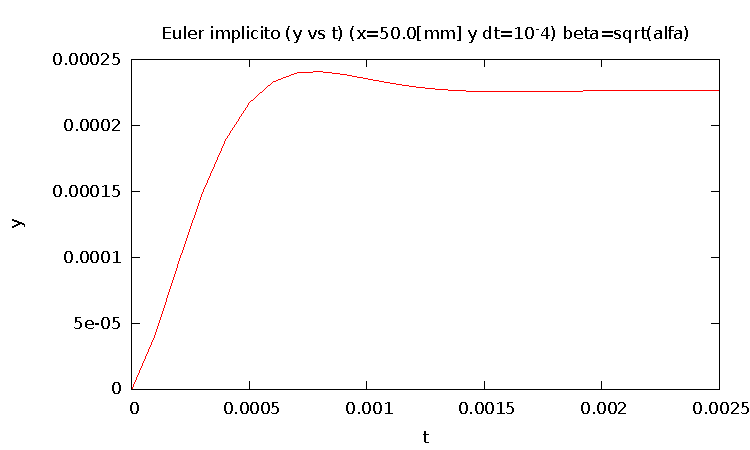
\includegraphics{./parte3/graficos/grafico_euler_S1_y_b1.pdf}
		\caption{Grafico de $y$ vs $t$ empleando un esquema de integración de Euler Implícito. $x=0.5[mm]$ y $\Delta t=10^{-4}$} 
		\label{fig:eulerS1b1_y}
	\end{subfigure}
	
	\begin{subfigure}[b]{0.8\textwidth}
		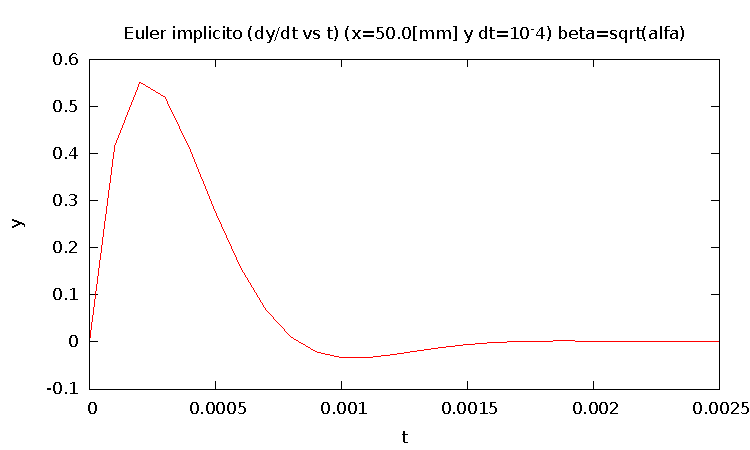
\includegraphics{./parte3/graficos/grafico_euler_S1_dy_b1.pdf}
		\caption{Grafico de $dy/dt$ vs $t$ empleando un esquema de integración de Euler Implícito. $x=0.5[mm]$ y $\Delta t=10^{-4}$} 
		\label{fig:eulerS1b1_dy}
	\end{subfigure}
\caption{Simulación 1: Solución numérica empleando Euler Implícito para $\beta=\sqrt{\alpha}$ } \label{euler_S1_b1}
\end{figure}
\end{center}

\begin{center}
\begin{figure} [H]
	\begin{subfigure}[b]{0.8\textwidth}
		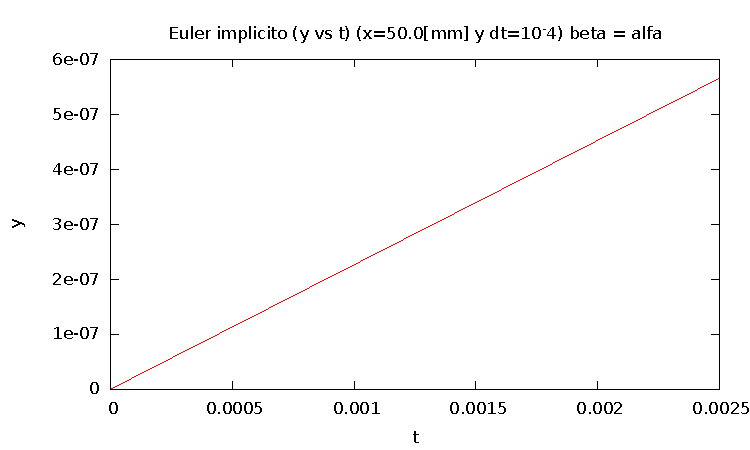
\includegraphics{./parte3/graficos/grafico_euler_S1_y_b2.pdf}
		\caption{Grafico de $y$ vs $t$ empleando un esquema de integración de Euler Implícito. $x=0.5[mm]$ y $\Delta t=10^{-4}$} 
		\label{fig:eulerS1b2_y}
	\end{subfigure}
	
	\begin{subfigure}[b]{0.8\textwidth}
		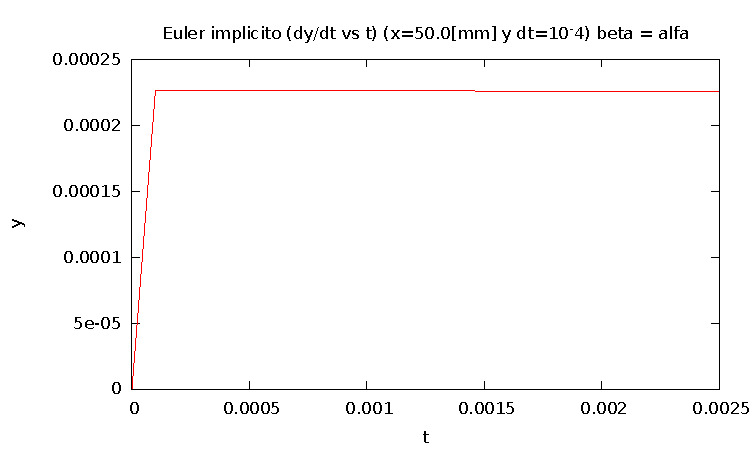
\includegraphics{./parte3/graficos/grafico_euler_S1_dy_b2.pdf}
		\caption{Grafico de $dy/dt$ vs $t$ empleando un esquema de integración de Euler Implícito. $x=0.5[mm]$ y $\Delta t=10^{-4}$} 
		\label{fig:eulerS1b2_dy}
	\end{subfigure}
\caption{Simulación 1: Solución numérica empleando Euler Implícito para $\beta=\alpha$ } \label{euler_S1_b2}
\end{figure}
\end{center}

%--------------------------------------------------------------------------

%----------------------- FIGURAS SIMULACION 1 -----------------------------
%----------------------- 	CRANK NICOLSON -----------------------------

\begin{center}
\begin{figure} [H]
	\begin{subfigure}[b]{0.8\textwidth}
		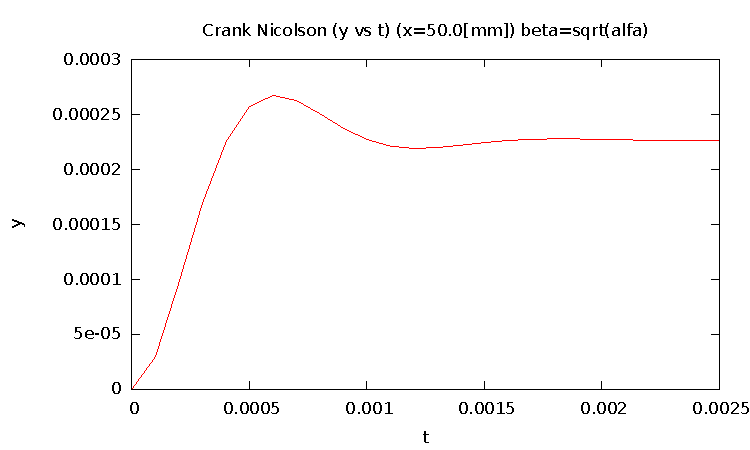
\includegraphics{./parte3/graficos/grafico_cn_S1_y_b1.pdf}
		\caption{Grafico de $y$ vs $t$ empleando un esquema de integración de Crank Nicolson. $x=0.5[mm]$ y $\Delta t=10^{-4}$} 
		\label{fig:cnS1b1_y}
	\end{subfigure}
	
	\begin{subfigure}[b]{0.8\textwidth}
		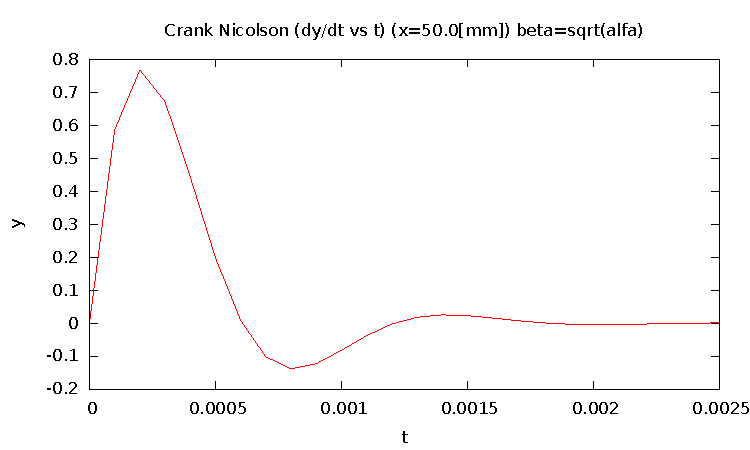
\includegraphics{./parte3/graficos/grafico_cn_S1_dy_b1.pdf}
		\caption{Grafico de $dy/dt$ vs $t$ empleando un esquema de integración de Crank Nicolson. $x=0.5[mm]$ y $\Delta t=10^{-4}$} 
		\label{fig:cnS1b1_dy}
	\end{subfigure}
\caption{Simulación 1: Solución numérica empleando Crank Nicolson para $\beta=\sqrt{\alpha}$ } \label{cn_S1_b1}
\end{figure}
\end{center}

\begin{center}
\begin{figure} [H]
	\begin{subfigure}[b]{0.8\textwidth}
		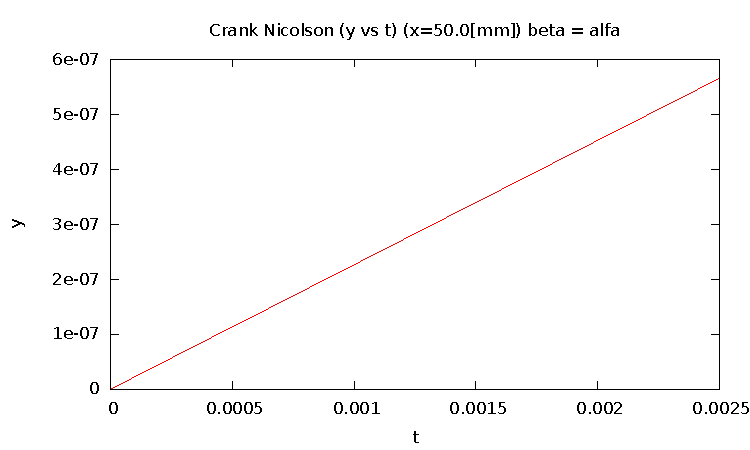
\includegraphics{./parte3/graficos/grafico_cn_S1_y_b2.pdf}
		\caption{Grafico de $y$ vs $t$ empleando un esquema de integración de Crank Nicolson. $x=0.5[mm]$ y $\Delta t=10^{-4}$} 
		\label{fig:cnS1b2_y}
	\end{subfigure}
	
	\begin{subfigure}[b]{0.8\textwidth}
		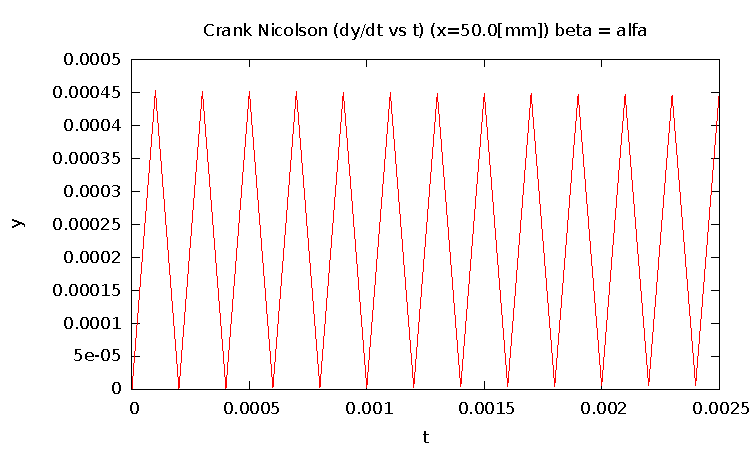
\includegraphics{./parte3/graficos/grafico_cn_S1_dy_b2.pdf}
		\caption{Grafico de $dy/dt$ vs $t$ empleando un esquema de integración de Crank Nicolson. $x=0.5[mm]$ y $\Delta t=10^{-4}$} 
		\label{fig:cnS1b2_dy}
	\end{subfigure}
\caption{Simulación 1: Solución numérica empleando Crank Nicolson para $\beta=\sqrt{\alpha}$ } \label{cn_S1_b2}
\end{figure}
\end{center}

%--------------------------------------------------------------------------

%----------------------- FIGURAS SIMULACION 2 -----------------------------
%----------------------- 	EULER IMPLICITO  -----------------------------

\begin{center}
\begin{figure} [H]
	\begin{subfigure}[b]{0.8\textwidth}
		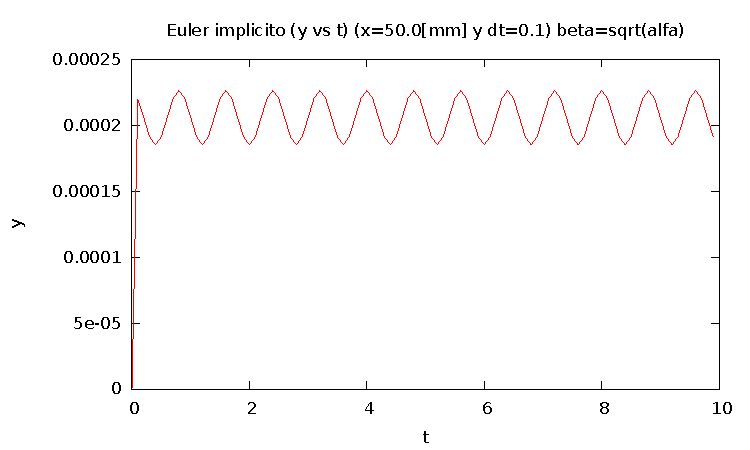
\includegraphics{./parte3/graficos/grafico_euler_S2_y_b1.pdf}
		\caption{Grafico de $y$ vs $t$ empleando un esquema de integración de Euler Implícito. $x=0.5[mm]$ y $\Delta t=0.1$} 
		\label{fig:eulerS2b1_y}
	\end{subfigure}
	
	\begin{subfigure}[b]{0.8\textwidth}
		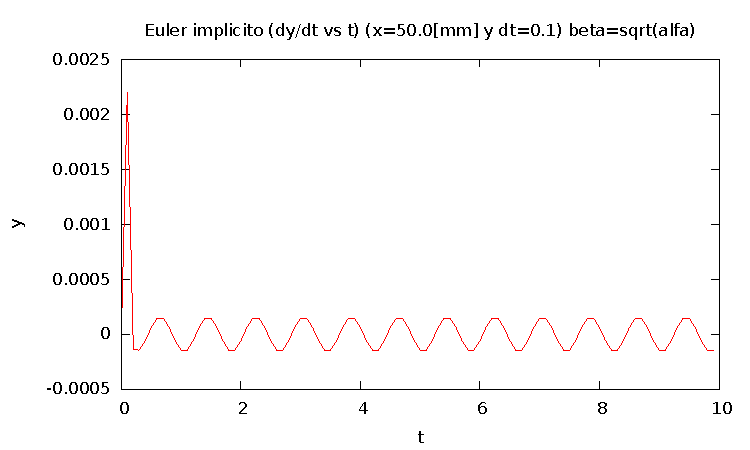
\includegraphics{./parte3/graficos/grafico_euler_S2_dy_b1.pdf}
		\caption{Grafico de $dy/dt$ vs $t$ empleando un esquema de integración de Euler Implícito. $x=0.5[mm]$ y $\Delta t=0.1$}  
		\label{fig:eulerS2b1_dy}
	\end{subfigure}
\caption{Simulación 2: Solución numérica empleando Euler Implícito para $\beta=\alpha$}
\end{figure}
\end{center}

\begin{center}
\begin{figure} [H]
	\begin{subfigure}[b]{0.8\textwidth}
		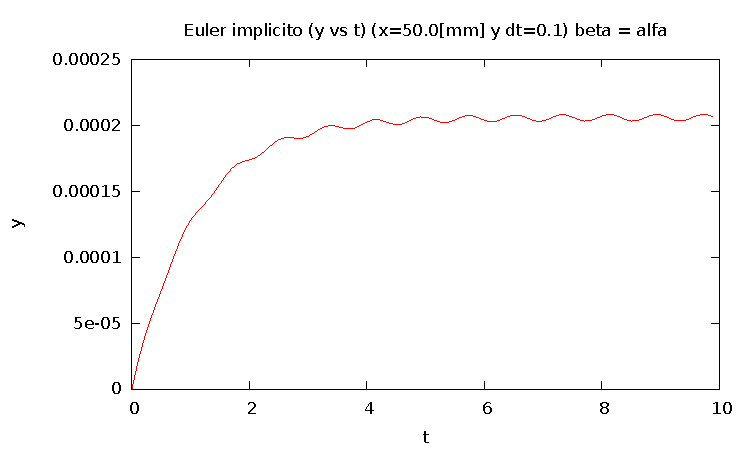
\includegraphics{./parte3/graficos/grafico_euler_S2_y_b2.pdf}
		\caption{Grafico de $y$ vs $t$ empleando un esquema de integración de Euler Implícito. $x=0.5[mm]$ y $\Delta t=0.1$} 
		\label{fig:eulerS2b2_y}
	\end{subfigure}
	
	\begin{subfigure}[b]{0.8\textwidth}
		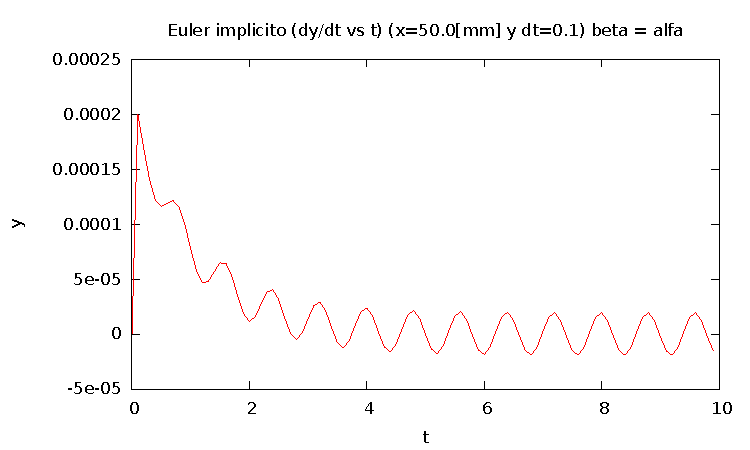
\includegraphics{./parte3/graficos/grafico_euler_S2_dy_b2.pdf}
		\caption{Grafico de $dy/dt$ vs $t$ empleando un esquema de integración de Euler Implícito. $x=0.5[mm]$ y $\Delta t=0.1$} 
		\label{fig:eulerS2b2_dy}
	\end{subfigure}
\caption{Simulación 2: Solución numérica empleando Euler Implícito para $\beta=\sqrt{\alpha}$}
\end{figure}
\end{center}

%--------------------------------------------------------------------------

%----------------------- FIGURAS SIMULACION 2 -----------------------------
%-----------------------	CRANK NICOLSON -----------------------------

\begin{center}
\begin{figure} [H]
	\begin{subfigure}[b]{0.8\textwidth}
		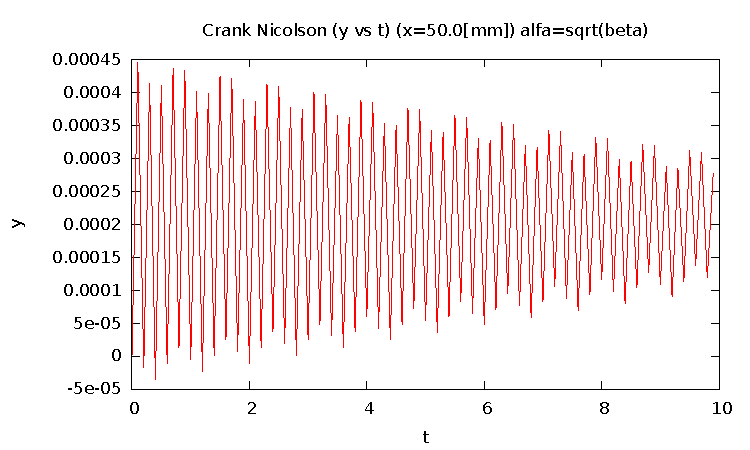
\includegraphics{./parte3/graficos/grafico_cn_S2_y_b1.pdf}
		\caption{Grafico de $y$ vs $t$ empleando un esquema de integración de Crank Nicolson. $x=0.5[mm]$ y $\Delta t=0.1$}  
		\label{fig:cnS2b1_y}
	\end{subfigure}
	
	\begin{subfigure}[b]{0.3\textwidth}
		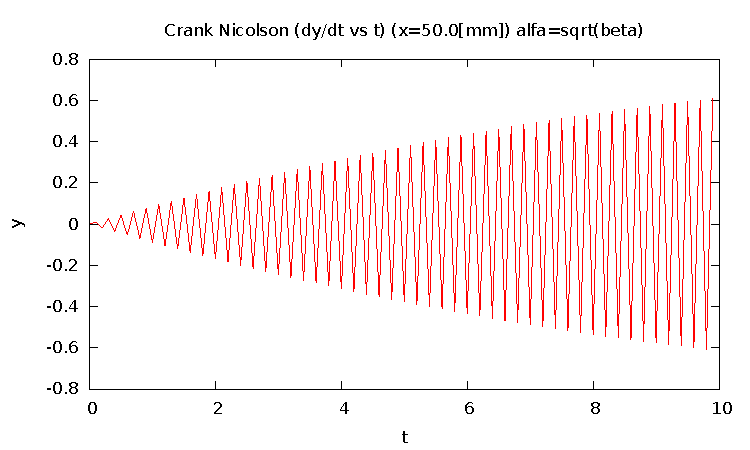
\includegraphics{./parte3/graficos/grafico_cn_S2_dy_b1.pdf}
		\caption{Grafico de $dy/dt$ vs $t$ empleando un esquema de integración de Crank Nicolson. $x=0.5[mm]$ y $\Delta t=0.1$}   
		\label{fig:cnS2b1_dy}
	\end{subfigure}
\caption{Simulación 2: Solución numérica empleando Crank Nicolson para $\beta=\alpha$}
\end{figure}
\end{center}

\begin{center}
\begin{figure} [H]
	\begin{subfigure}[b]{0.8\textwidth}
		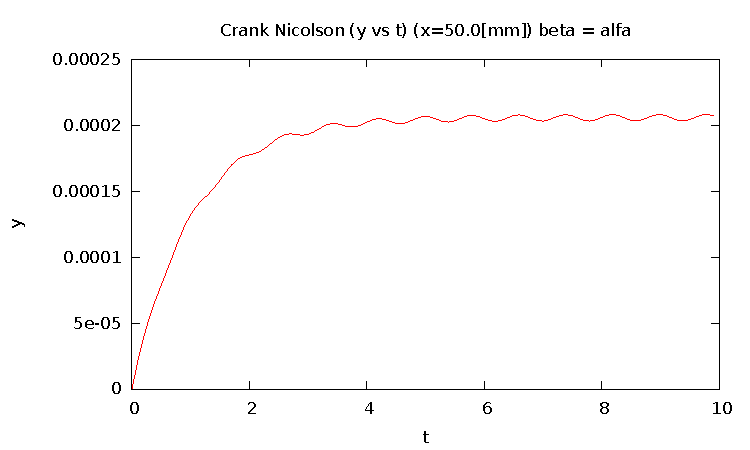
\includegraphics{./parte3/graficos/grafico_cn_S2_y_b2.pdf}
		\caption{Grafico de $y$ vs $t$ empleando un esquema de integración de Crank Nicolson. $x=0.5[mm]$ y $\Delta t=0.1$}  
		\label{fig:cnS2b2_y}
	\end{subfigure}
	
	\begin{subfigure}[b]{0.8\textwidth}
		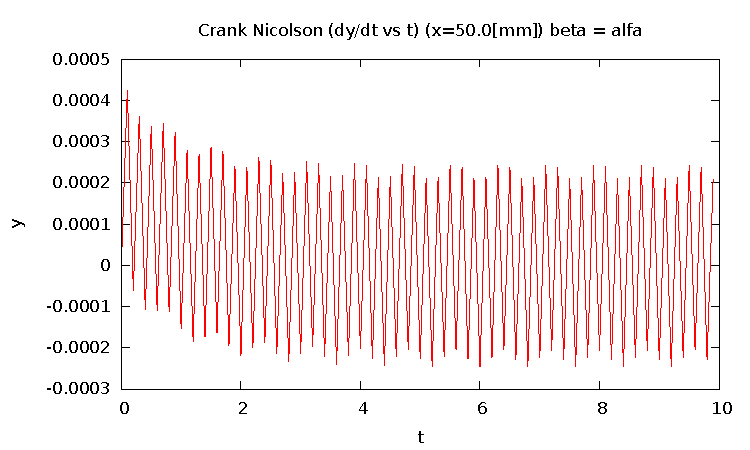
\includegraphics{./parte3/graficos/grafico_cn_S2_dy_b2.pdf}
		\caption{Grafico de $dy/dt$ vs $t$ empleando un esquema de integración de Crank Nicolson. $x=0.5[mm]$ y $\Delta t=0.1$} 
		\label{fig:cnS2b2_dy}
	\end{subfigure}
\caption{Simulación 2: Solución numérica empleando Crank Nicolson para $\beta=\sqrt{\alpha}$}
\end{figure}

\end{center}

%------------------------------------------------------------------------ 

\newpage
%Estudio del comportamiento mecánico de una arteria

\subsection{Parte 2: Un modelo hiperbólico para la interacción de la sangre con la pared}

Si para el mismo fenomeno descrito en la Parte 1 no se desprecia la interacción axial entre los anillos, entonces la ecuación (\ref{PROBLEMA_PARTE_2}) se modifica resultado en,

\begin{equation} \label{PROBLEMA_PARTE_2_2}
\dfrac{\partial^2 u}{\partial t^2} - \gamma^2 \dfrac{\partial^2 u}{\partial x^2} = f \hspace{0,5cm} x \in ] \alpha , \beta [
\end{equation}

Se denota la coordenada longitudinal $x$. $\sigma_x$ es la componente radial del esfuerzo axial y $L$ es el largo del cilindro considerado. Despreciando el factor de $y$ de la ecuación (\ref{PROBLEMA_PARTE_2_2}) y considerando $p-p_0 = f$ entonces se obtiene la ecuación de onda en una dimensión

\begin{equation} \label{E_ONDA}
\dfrac{\partial^2 u}{\partial t^2} - \gamma \dfrac{\partial^2 u}{\partial x^2} = f
\end{equation}

Se emplean los esquemas de Leap-Frog y Newmark para discretizar la ecuación anterior.

\subsubsection{Simulación 1: Leap-Frog}

El termino fuente utilizado para la simulación es $ f = ( 1 + \pi^2 \gamma^2 ) e^{-t} sin( \pi x ) $. Empleando un esquema de diferencias centradas en el espacio,

\begin{equation}
\dfrac{ \partial^2 u }{ \partial t^2 } = \gamma^2 \dfrac{ u_{j+1}^n - 2 u_j^n + u_{j-1}^n }{ \Delta x ^2} + 
 ( 1 + \pi^2 \gamma^2 ) e^{-t} sin( \pi x_j ) 
\end{equation}

Se utiliza un esquema de integración de Leap-Frog,

\begin{equation}
u^{n+1}_j - 2u^n_j + u^{n-1} = (\gamma \lambda)^2 ( u^n_{j-1} -2 u^n_j + u^n_{j+1} ) + f^n_j
\end{equation}

donde $\lambda=\dfrac{\Delta t}{\Delta x}$

Se estudia la estabilidad del método: 

\subsubsection*{Discretización espacial}

Se realiza una descomposición modal

\begin{align*}
S e ^ { i k_j p \Delta x } &= \dfrac{\gamma^2}{\Delta x^2} \left( e ^ { i k_j (p+1) \Delta x } - 2 e ^ { i k_j p \Delta x } + e ^ { i k_j (p-1) \Delta x } \right) \\
&= \underbrace{\dfrac{2 \gamma^2}{\Delta x^2} \left( cos(k_j \Delta x) - 1 \right)}_{\Omega_j} e ^ { i k_j p \Delta x}
\end{align*}

Es decir,

\begin{equation} \label{OMEGA_LF}
\Omega_j = \dfrac{2 \gamma^2}{\Delta x^2} \left( cos(k_j \Delta x) - 1 \right)
\end{equation}

Notar que $\Omega = \Re(\Omega_j)$. Se debe cumplir que

\begin{equation}
\Re(\Omega_j) \leq 0
\end{equation}

luego,

\begin{equation}
\Big| \dfrac{2 \gamma^2 }{ \Delta^2 } \leq 0
\end{equation}

\begin{equation}
\dfrac{-4 \gamma^2}{\Delta x^2} \leq \Re(\Omega_j) \leq 0
\end{equation}

\subsubsection*{Discretización temporal}

Estudia la estabilidad en el tiempo: se reemplaza $u_{j} = \omega$

\begin{equation}
\dfrac{\omega^{n+1} -2\omega^{n} + \omega^{n+1}}{\Delta t^2} = \vect{S} = \Omega_j \omega^n
\end{equation}

reeordenando

\begin{equation}
\omega^{n+1} - (\Omega_j \Delta t^2 +2) \omega^n + \omega^{n-1}
\end{equation}

utilizando $z_p$ (ver Sección ¿?, ecuación (¿?))

\begin{equation}
z_p^2 - \left( \Omega_j \Delta t^2 +2 \right) z_p + 1 = 0
\end{equation}

diviendo por $z_p$ (supuesto: $z_p \neq 0$, el estado transiente)

\begin{equation}
\left( \Omega_j \Delta t^2 + 2 \right) = \dfrac{1}{z_p} + z_p
\end{equation}

Se impone como solución $z_p = e^{i \theta}$ (notar que $|z_p| \leq 1$) . Reemplazando en la ecuación anterior,

\begin{equation}
\left( \Omega_j \Delta t^2 + 2 \right) = e^{i \theta} + e^{-i \theta} = 2 cos(\theta)
\end{equation}

La estabilidad se consigue acotando el lado izquierdo de la ecuación, obteniendo

\begin{equation}
-4 \leq \Re(\Omega_j \Delta t^2) \leq 0 
\end{equation}

reemplazando $\Omega_j$ obtenido de la ecuación (\ref{OMEGA_LF}) y considerando $\Omega_j = \Re (\Omega_j)$ resulta,

\begin{equation}
-4 \leq \dfrac{\gamma^2 \Delta t^2}{\Delta x^2} \left( cos(k_j \Delta x) - 1 \right)  \leq 0
\end{equation}

El criterio de estabilidad es

\begin{equation}
\dfrac{\gamma^2 \Delta t^2}{\Delta x^2} \leq 2
\end{equation}

$\gamma^2 \Delta t^2 / \Delta x^2 $ se puede interpretar como $(CFL)^2$ donde $CFL$ es el número de Courant-Friedrichs-Lewy

PENDIENTE -ESCRIBI LAS ECUACIONES, FALTA EXPLICARLAS !!!!!!!!!!!!!!!!

\subsubsection{Simulación 1: Newmark}

De la ecuacion (¿?) (Sección 1) se tiene $\partial u / \partial t = v$

\begin{equation}
\dfrac{\partial v}{\partial t} = \gamma ^2 \left[ \Theta \left( \dfrac{ u_{j+1}^{n+1} -2u_{j}^{n+1} + u_{j-1}^{n+1} }{\Delta x^2} \right) - (1-\Theta) \left( \dfrac{ u_{j+1}^{n} -2u_{j}^{n} + u_{j-1}^{n} }{\Delta x^2} \right) \right]
\end{equation} 

\subsubsection{Discretización espacial}

Se utiliza $\Theta=0.5$ (Esquema Crank Nicolson)

\begin{equation}
\dfrac{\partial v}{\partial t} = \left[ \left( \vect{S} e^{i k_j p \Delta x} \right)^{n+1} + \left( \vect{S} e^{i k_j p \Delta x} \right)^{n}  \right]
\end{equation}

Se resulve $(\vect(S))^n$

\begin{align*}
S e ^ { i k_j p \Delta x } &= \dfrac{\gamma^2}{2 \Delta x^2} \left( e ^ { i k_j (p+1) \Delta x } - 2 e ^ { i k_j p \Delta x } + e ^ { i k_j (p-1) \Delta x } \right) \\
&= \underbrace{\dfrac{\gamma^2}{\Delta x^2} \left( cos(k_j \Delta x) - 1 \right)}_{\Omega_j} e ^ { i k_j p \Delta x}
\end{align*}

es decir,

\begin{equation} \label{OMEGA_j}
\Omega_j = \dfrac{\gamma^2}{\Delta x^2} \left( cos(k_j \Delta x) - 1 \right)
\end{equation}

\begin{equation} \label{CONDICION_OMEGA_j_NM}
\dfrac{-2 \gamma^2}{\Delta x^2} \leq \Re(\Omega_j) \leq 0
\end{equation}

Se obtiene el mismo resultado para $(\vect(S))^{n+1}$, Sumando $(\vect(S))^{n+1} + (\vect(S))^{n}$ luego obtenemos la mismas ecuación obtenida en la discretización Leap-Frog. Por lo tanto, la condición de $\Re(\Omega_j')$ ($\Omega_j' = \Omega_j^{n+1} + \Omega_j^{n}$)

\begin{equation}
\dfrac{-4 \gamma^2}{\Delta x^2} \leq \Re(\Omega_j') \leq 0
\end{equation}

Como $u_j$ y $v_j$ emplean diferencias finitas centradas se obtienen los mismos valores propios de $\vect{S}$

\subsubsection*{Discretización temporal}

Se integra la ecuación $\partial v / \partial t$. Se utiliza la notación $v_j = \omega$

\begin{equation}
\dfrac{\omega^{n+1}-\omega^n}{\Delta t} = \Omega_j^{n+1} \omega^{n+1} + \Omega_j^{n} \omega^{n}
\end{equation}

agrupando términos

\begin{equation}
\omega^{n+1} = \underbrace{ \dfrac{1+\Omega_j \Delta t}{1-\Omega_j \Delta t} }_{z_p} \omega^n
\end{equation}

como $\Omega_j = \Re(\Omega_j)$, entonces

\begin{equation} \label{zp_nm_v}
z_p = \dfrac{ 1 + \Omega_j }{ 1-\Omega_j}
\end{equation}

tomando en cuenta la condición \ref{CONDICION_OMEGA_j_NM} se verifica que

\begin{equation}
-1 \leq z_p \leq 1
\end{equation}




%----

\subsection{Atractor de Lorenz}
%ATRACTOR DE LORENZ
El sistema de ecuaciones de Lorenz es un ejemplo de un sistema de ecuaciones diferenciales de orden 1, tridimensional, no lineal, que tiene un comportamiento caótico para algunos valores de sus parámetros. Este sistema de ecuaciones permite modelar los rollos de convección que se producen en la atmosfera terrestre. Es un modelo simplificado de la convección de Rayleigh-Benard (ecuaciones de Navier-Stokes con hipótesis de Boussinesq).
\begin{equation}
\left\{ 
\begin{matrix}
dx/dt =& Pr (y(t) - x(yt)) \\
dy/dt =& Ra x(t) - y(t) - x(t)z(t) \\
dz/dt =& x(t) y(t) - \beta z(t)
\end{matrix} \right.
\end{equation}
Donde $Pr$ es el número de Prandtl y $Ra$ es el número de Rayleigh. Las variables dinámicas $x$, $y$ y $z$ represetan el estado del sistema a cada instante $t$:

\begin{itemize}
\item x(t) es proporcional a la intensidad del movimiento de convección  
\item y(t) es proporcional a la diferencia de temperatura entre las corrientes ascendentes y descendentes
\item z(t) es proporcional a la diferencia entre el perfil vertical de temperatura y un perfil vertical de temperatura lineal
\end{itemize}

Los sistemas dinámicos son sistemas que son función del tiempo. Que sea caótico significa que varia de manera no lineal y a su vez que el sistema presenta sensibilidad a frente a los parámetros entrada. Además presentan un comportamiento oscilante, pudiendo ser periodico o no periodico. \\

\subsubsection{Parte 1}
Las Figuras \ref{lorenz1} y \ref{lorenz2} reproducen los gráficos del articulo \textit{Deterministic Nonperiodic Flow} de Lorenz
\begin{figure} [H]
\begin{center}
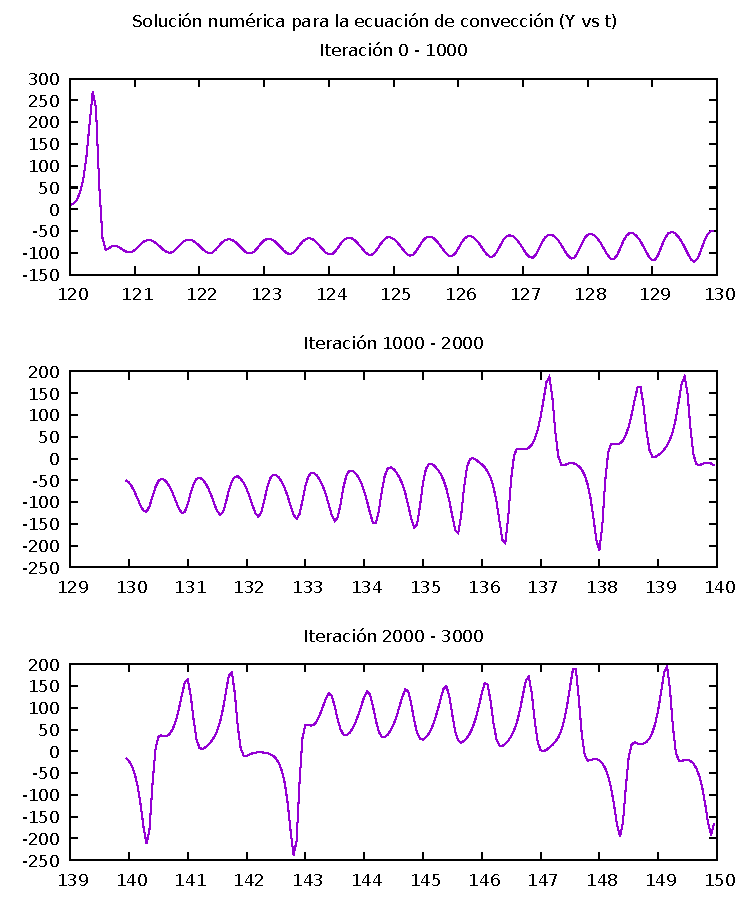
\includegraphics[width=0.8\textwidth]{./parte4/graficos/FIGURA1.pdf}
\caption{} \label{lorenz1}
\end{center}
\end{figure}

\begin{figure} [H]
\begin{center}
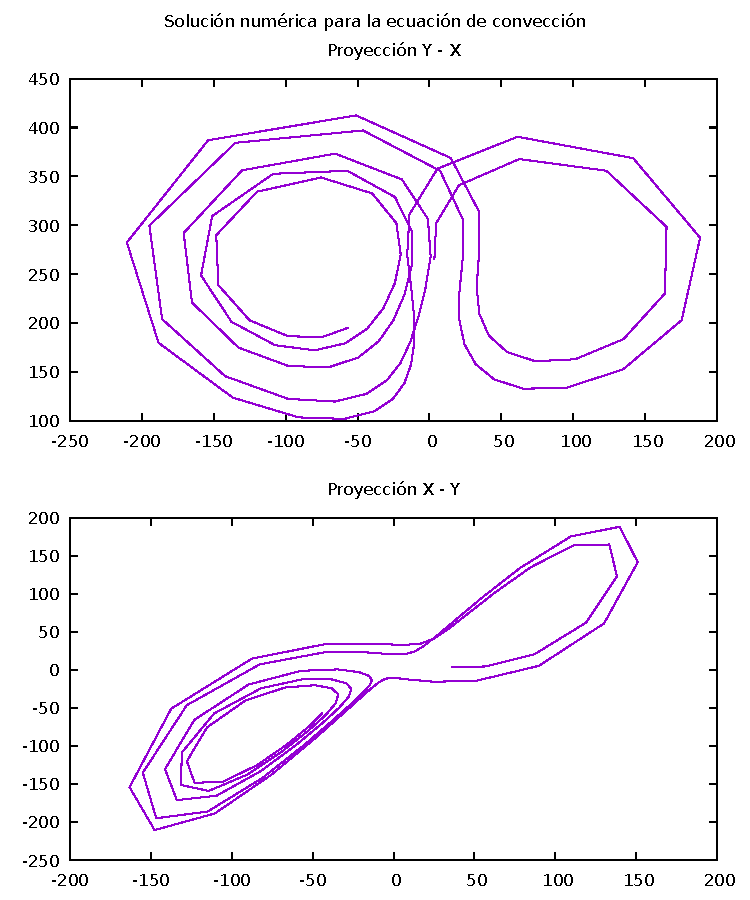
\includegraphics[width=0.8\textwidth]{./parte4/graficos/FIGURA2.pdf}
\caption{} \label{lorenz2}
\end{center}
\end{figure}

%---------------------------

\subsubsection{Parte 2}

Se grafica la solución a la ecuación de convección utilizando los siguientes valores: $Pr=10$, $\beta= 8/3$ y $Ra = 0.5 \, , \, 10 , \, 28$ 

\begin{figure} [H]
\begin{center}
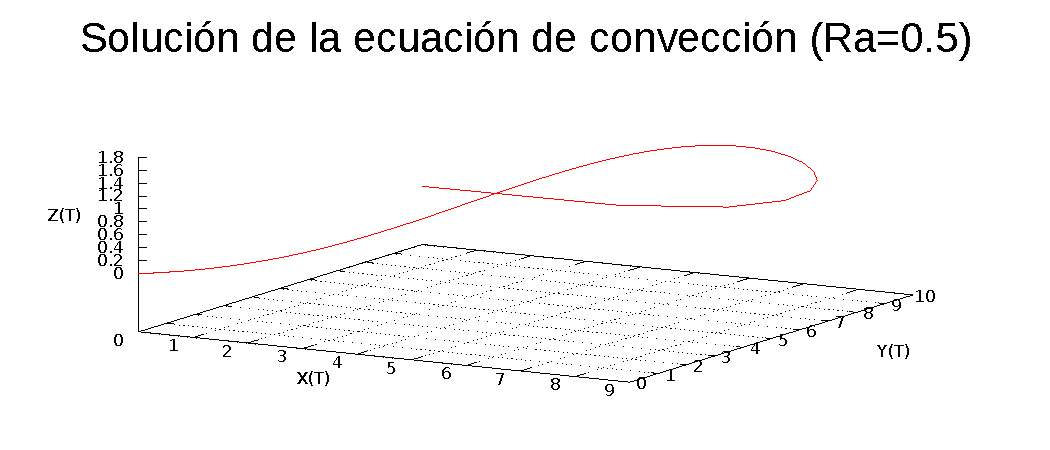
\includegraphics[width=0.8\textwidth]{./parte4/graficos/grafico_P3_3d_ra05.pdf}
\caption{}
\end{center}
\end{figure}

\begin{figure} [H]
\begin{center}
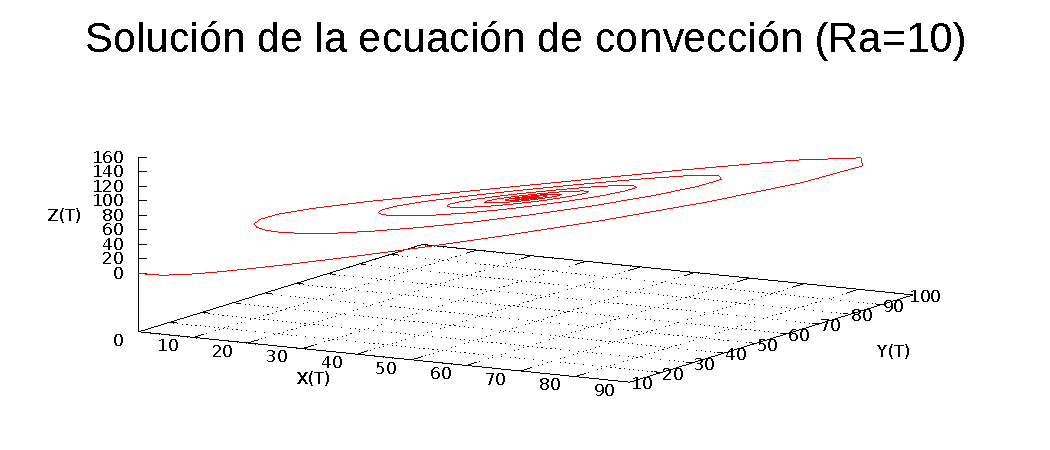
\includegraphics[width=0.8\textwidth]{./parte4/graficos/grafico_P3_3d_ra10.pdf}
\caption{}
\end{center}
\end{figure}

\begin{figure} [H]
\begin{center}
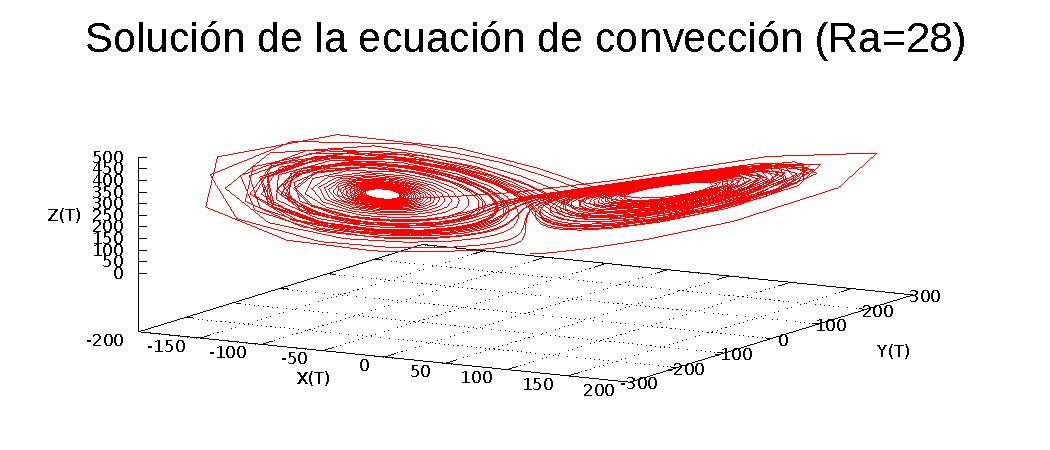
\includegraphics[width=0.8\textwidth]{./parte4/graficos/grafico_P3_3d_ra28.pdf}
\caption{}
\end{center}
\end{figure}

%---------------------------

\subsubsection{Parte 3}
Haciendo variar paulatinamente $Ra$ entre 0 y 30

\begin{figure} [H]
\hspace{-1cm} 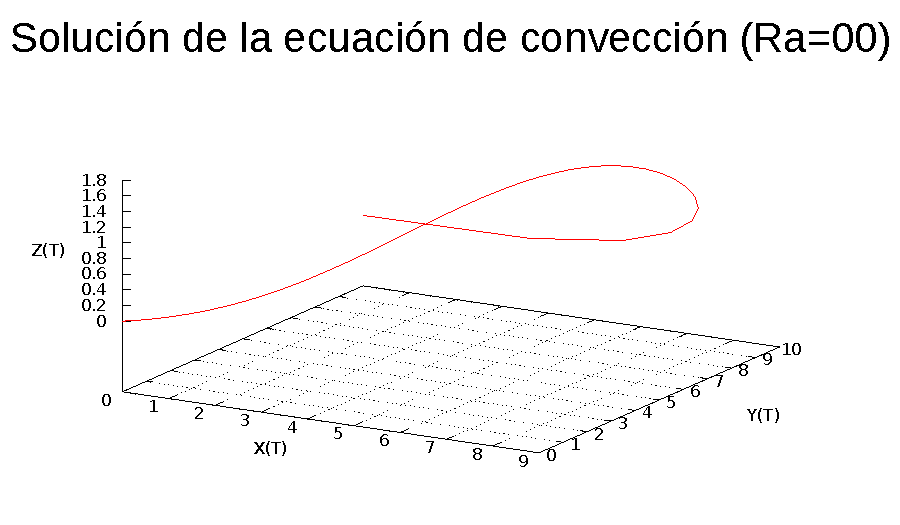
\includegraphics[width=0.6\textwidth]{./parte4/graficos/grafico_P3_3d_ra00.pdf}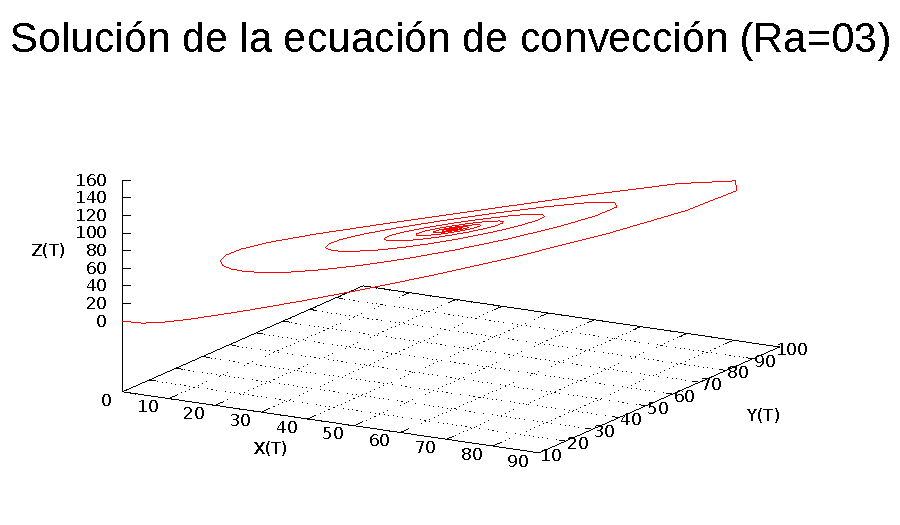
\includegraphics[width=0.6\textwidth]{./parte4/graficos/grafico_P3_3d_ra03.pdf}
\caption{} 
\end{figure}

\begin{figure} [H]
\hspace{-1cm} 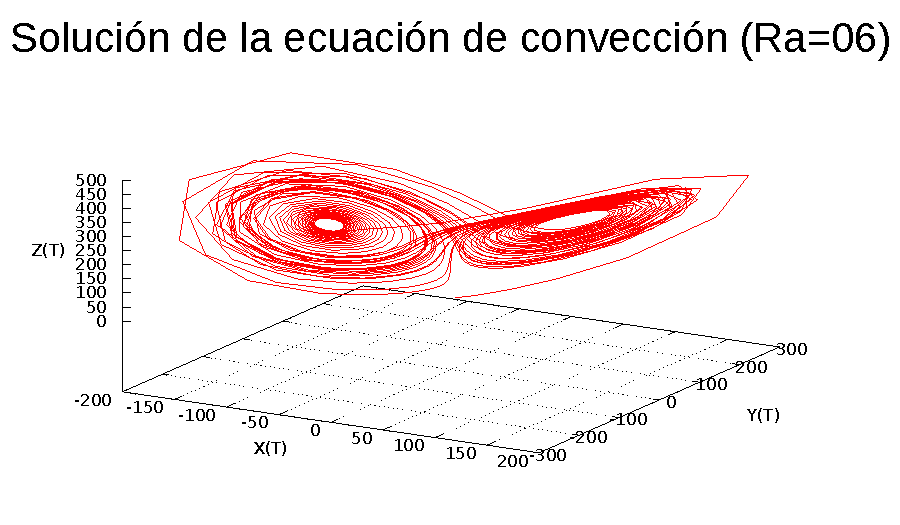
\includegraphics[width=0.6\textwidth]{./parte4/graficos/grafico_P3_3d_ra06.pdf}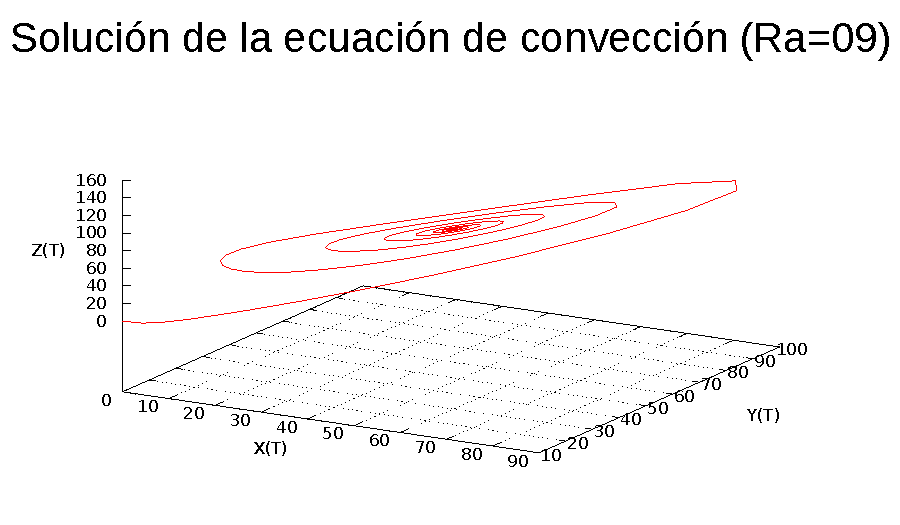
\includegraphics[width=0.6\textwidth]{./parte4/graficos/grafico_P3_3d_ra09.pdf}
\caption{} 
\end{figure}

\begin{figure} [H]
\hspace{-1cm} 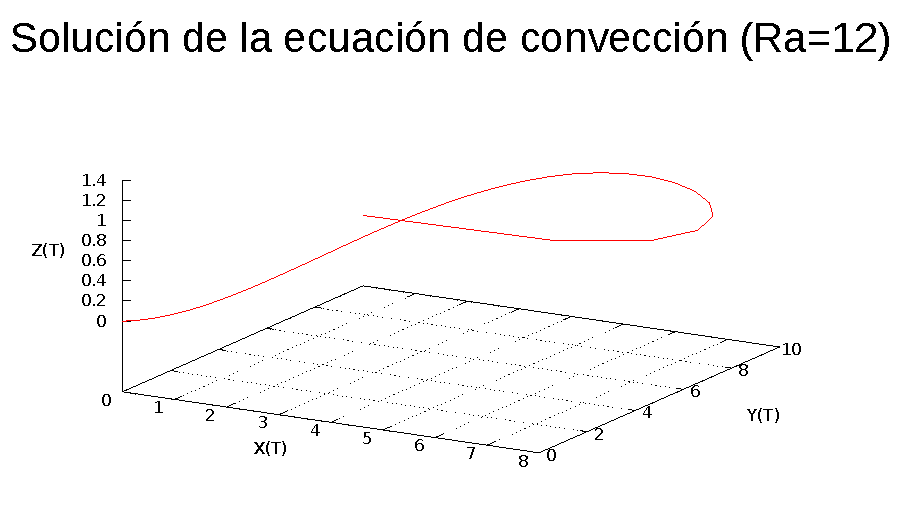
\includegraphics[width=0.6\textwidth]{./parte4/graficos/grafico_P3_3d_ra12.pdf}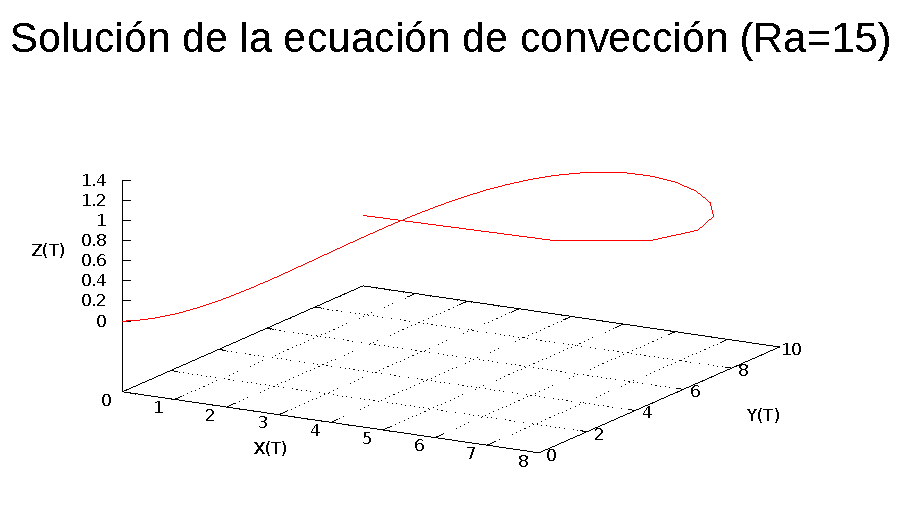
\includegraphics[width=0.6\textwidth]{./parte4/graficos/grafico_P3_3d_ra15.pdf}
\caption{} 
\end{figure}

\begin{figure} [H]
\hspace{-1cm} 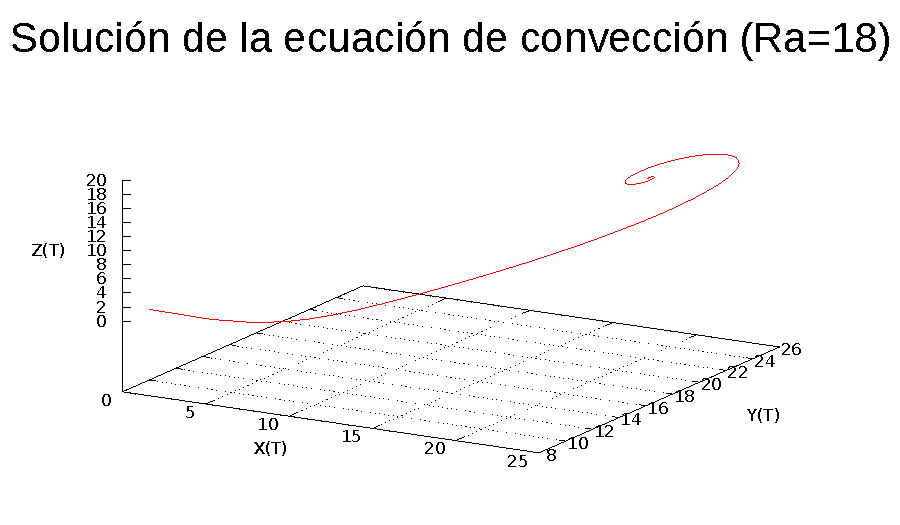
\includegraphics[width=0.6\textwidth]{./parte4/graficos/grafico_P3_3d_ra18.pdf}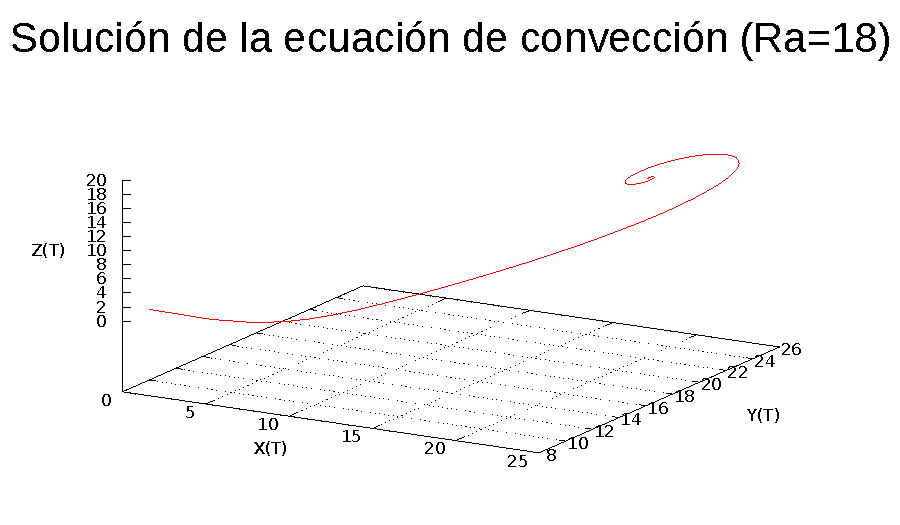
\includegraphics[width=0.6\textwidth]{./parte4/graficos/grafico_P3_3d_ra18.pdf}
\caption{} 
\end{figure}

\begin{figure} [H]
\hspace{-1cm} 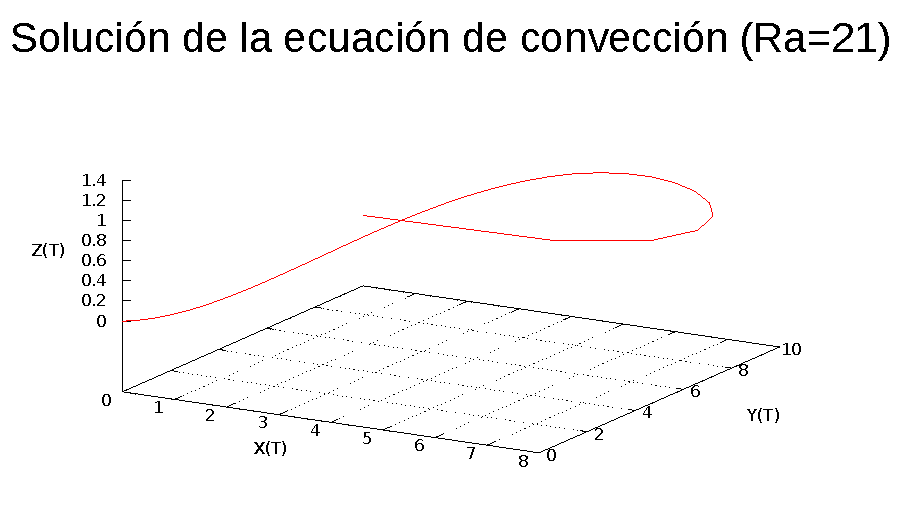
\includegraphics[width=0.6\textwidth]{./parte4/graficos/grafico_P3_3d_ra21.pdf}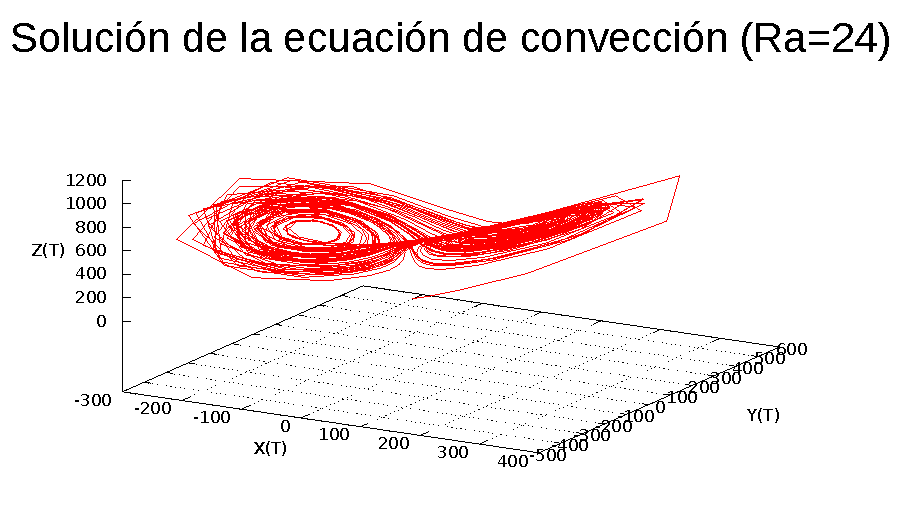
\includegraphics[width=0.6\textwidth]{./parte4/graficos/grafico_P3_3d_ra24.pdf}
\caption{} 
\end{figure}

\begin{figure} [H]
\hspace{-1cm} 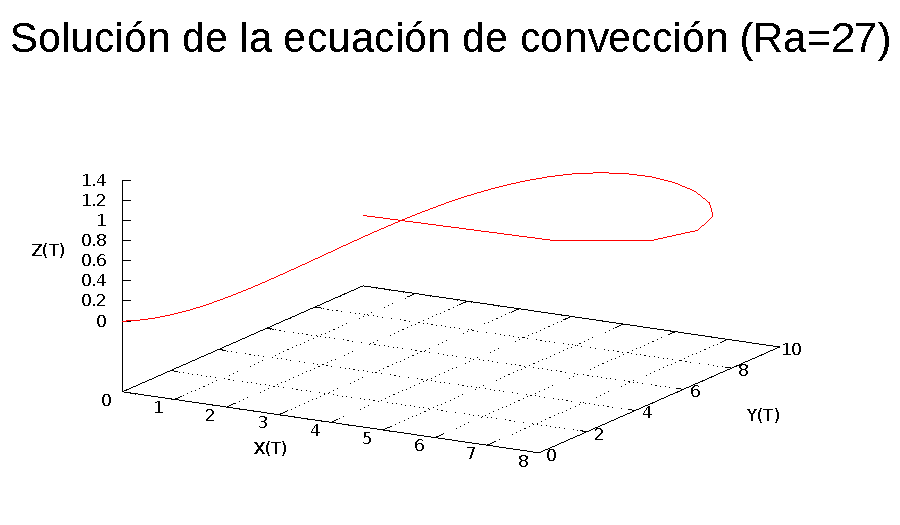
\includegraphics[width=0.6\textwidth]{./parte4/graficos/grafico_P3_3d_ra27.pdf}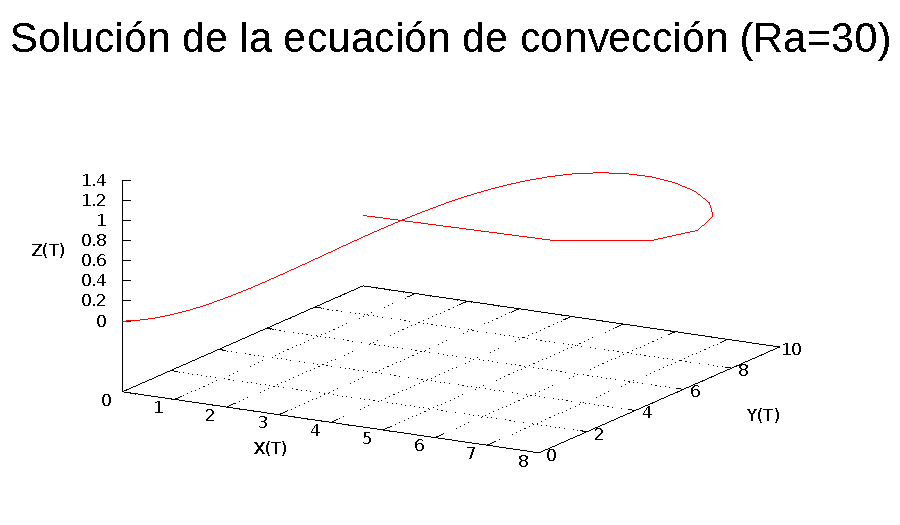
\includegraphics[width=0.6\textwidth]{./parte4/graficos/grafico_P3_3d_ra30.pdf}
\caption{} 
\end{figure}

\newpage
%---------------------------------------------

\section{Conclusiones y Observaciones}

\paragraph{Ejercicios en Fortran} Se estudió la relevancia del parámetro \texttt{precision} en la implementación de las rutinas. En el Ejercicio 1 se observa que para un número determinado de operaciones la precisión representa un freno debido a la debil resolución numérica, es decir, para una cantidad de decimales que se supera la cantidad de cifras significativas no alteran al objeto, por que la operación virtualmente no ocurre. \\

El caso contrario ocurre en el Ejercicio 2. Se trabajó con número enteros y reales y se observó el comportamiento de ambos al representar la serie Fibonacci. La inestabilidad se presenta cuando la operación numérica produce un número de mayor tamaño del que la memoria asignada puede contemplar. Cuando sucede esto ocurre una asignación de memoria que no representa ninguna operación, es decir, se obtiene un resultado aleatorio sin significancia física ni matematica. \\

El Ejercicio 3 se implementa una subrutina que permite realizar la operación de multiplicación matricial. Se implementa una rutina que realiza la multiplicación cuando las dimensiones de los dos factores son consistentes con los de la operación. La rutina implementada trabaja con un parametro $l$ de tal manera que $l=0$ cuando la operación en satisfactoria, y $l=1$ cuando ocurre un error. Este tipo de consideración son relevantes al momento de implementar algoritmos: Una práctica aconsejable al momento de programar es establercer detenciones o \textit{flags} que permitan identificar cuando ocurre una operación indeseado o se obtienen resultado malogrados. De esta manera se puede identificar facilmente el problema, con los tiempo de revisión y tiempo de cómputo malgastado. \\

\paragraph{Estudio del comportamiento de una arteria. Parte 1} 
Se implementó una rutina de integración de Euler Implícito y una de Crank Nicolson para la resolución de la ecuación (\ref{PROBLEMA_PARTE2_CORREGIDO}).
$$ {y}' = \vect{A} \vec{y} + b(x,t)$$
 Se observa que es una ecuación diferencial ordinaria, donde el término fuente es el único término que es función de la variable espacial $x$. En este caso la descomposición modal $\vect{A} V^{(j)} = \Omega_j V^{(j)}$ tiene una significancia distinta a la descomposición obtenida de un esquema de diferencias finitas: En el primer caso los valores propios están asocidos a la naturaleza del fenomeno (o bien, a la clasifica de la EDO), mientras que en el segundo caso está asociado a la estabilidad de la discretización. \\
 
Euler representa un esquema disipativo de orden 1, mientras que Crank Nicolson es un esquema dispersivo de orden 2. Al comparar las solución se observa que ambos métodos arrojan resultados distintos para un mismo problema. Además para un el caso $\beta=\sqrt{\alpha}$ se obtiene una solución con un término transiente oscilatorio. Se obtuvo numericamente que el método de Crank Nicolson es un esquema dispersivo. En este caso una solución que presenta oscilaciones se resuelve de manera desfavorable con ciertos métodos, particularmente, el método de Crank Nicolson, al ser un esquema dispersivo, agrega errores claramente visibles.

\paragraph{Estudio del comportamiento de una arteria. Parte 2} 
Se resolvió la ecuación de onda mediante los métodos de Leap-Frog y Newmark. Ambos métodos son \textit{three level scheme} ya que la discretización de la derivada temporal requiere de 3 valores $n$, $n+1$ y $n+2$. Ambos esquemas son de orden 2, luego, se espera que la tabla de convergencia \ref{tabla_lf_nm} se obtuviesen valores cercanos a 2. Discrepancias en los resultados pueden tener algunas posibles explicaciones:
\begin{itemize}
\item Iniciación (condiciones iniciales), Para obtener esta tabla se fue necesario conocer la función analítica para calcular los errores. Sin embargo se utilizó la condición inicial $u^0_j$ y se aproximó $u^1_j$ mediante diferencias finitas hacia adelante.
\item Para la resolución de Newmark se implementó una subrutina \textit{solver} que permite invertir la matriz que acompaña las incognitas $u^{n+1}$ mediante factorización pivoteada LU. Este método no es el más efectivo y puede incluir errores numéricos. Ya que se trata de un sistema tridiagonal (matriz sparse o con varios elementos nulos) lo mejor es utilizar un subrutina que trabaje que estos valores no nulos. Metodos más eficientes pueden verse en \cite{inv}, o utilizando librerias especializadas como LAPACK-BLAS.
\end{itemize}


\newpage
%---------------------------------------------

\section{Codigos implementados}
\subsection{Ejercicios en Fortran}
\subsubsection{Ejercicio 1}
\begin{lstlisting}
program EJERCICIOS_EN_FORTRAN_1
	!-------------------------------------------
	!PREAMBULO
	integer::i,inf,contador
	real(kind=4)::A !simple precision
	real(kind=8)::B,error !doble precision
	character(len=22)::datos_p1='./datos/datos_p1.dat'
	character(len=22)::datos_pe='./datos/datos_p1_error.dat'
	!-------------------------------------------
 	
 	!simple y doble precisión
	A=1._4
	B=1._8
	inf=4000000
	contador=1
	
	! los datos generados se exportan al directorio
	! ./datos/datos_p1.dat
	open(unit=10,file=datos_p1,action='write')
	do i=2,inf
		!contador
		contador = contador + 1
		!desarrollo de la serie
		A = A + ( 1._4 / real(i,kind=4) )
		B = B + ( 1._8 / real(i,kind=8) )
		error = (B-real(A,kind=8))/B
		!cada 1000 operaciones exportar datos
		if ( contador .eq. 10000 ) then
			if ( i .gt. 250000 ) then
				write(10,*) i, A, B, error
			end if
			contador=0
		end if
	end do 
	close(unit=10)
	
	!-------------------------------------------
	
	! se grafica la curva en el directorio
	! ./graficos/graficos_p1.dat
	call system ( ' cd ./gnuplot && gnuplot plot_p1_1.txt ' )
	
	!-------------------------------------------
	
end program
\end{lstlisting}

\newpage
\subsubsection{Ejercicio 2}
\begin{lstlisting}
program EJERCICIOS_EN_FORTRAN_2
	!-------------------------------------------
	!PREAMBULO
	integer::n,u0,u1,u2,j
	real(kind=8)::u0_r,u1_r,u2_r
	character(len=22)::datos_p2_1='./datos/datos_p2_1.dat'
	character(len=22)::datos_p2_2='./datos/datos_p2_2.dat'
	!-------------------------------------------

	!se calcula la serie para número enteros
	n=100
	u0=0 ; u1=1
	open(unit=10,file=datos_p2_1,action='write')
		write(10,*)0,u0
		write(10,*)1,u1
		do j=2,n
			u2=u0+u1
			write(10,*)j,u2
			u0=u1
			u1=u2
		end do
	close(unit=10)
	
	!se calcula la serie para número reales d. precision
	n=1500
	u0_r = 0._8 ; u1_r = 1._8
	open(unit=10,file=datos_p2_2,action='write')
		write(10,*)0,u0_r
		write(10,*)1,u1_r
		do j=2,n
			u2_r = u0_r + u1_r
			write(10,*) j , u2_r
			u0_r = u1_r
			u1_r = u2_r
		end do
	close(unit=10)
	
	!-------------------------------------------
	
	! se grafica la curva en el directorio
	! ./graficos/graficos_p1.dat
	call system ( ' cd ./gnuplot && gnuplot plot_p1_2.txt ' )
\end{lstlisting}

\newpage
\subsubsection{Ejercicio 3}
\begin{lstlisting}
!EL PROGRAMA EJECUTA DOS OPERACIONES DE EJEMPLO
!COMO SE MUESTRA A CONTINUACION

!PRIMER CASO AxB=C (DIMENSIONES CONSISTENTES)

!	A =	1	2	3	4
!		5	6	7	8
!		9	10	11	12
	
!	B =	1	2
!		3	4
!		5	6
!		7	8
	
!SEGUNDO CASO AxD (DIMENSIONES INCOSITENTES)

!	A =	1	2	3	4
!		5	6	7	8
!		9	10	11	12
	
!	D =	1	2
!		3	4
!		5	6

program EJERCICIOS_EN_FORTRAN_3
	!-------------------------------------------
	!INTERFACE
	implicit none
	interface
		subroutine matrix_mult(A,B,C,i)
		real(kind=4),dimension(:,:),intent(in)::A,B
		real(kind=4),dimension(:,:),intent(out)::C
		integer,intent(out)::i
		end subroutine
	end interface
	!-------------------------------------------
	!PREAMBULO
	
	!PREGUNTA 3
	integer::k,i,tmp,tmp_v(2)
	real(kind=4) :: A(3,4),B(4,2),D(3,2)
	real(kind=4),allocatable :: C(:,:)
	
	!-------------------------------------------
	
	!presentacion en pantalla
	write(*,*) '---------------------'
	write(*,*) 'EJERCICIOS_EN_FORTRAN_3'
	write(*,*) 'codigo		: P1_3.f90'
	write(*,*) 'ejecutable	: P1_3'
	write(*,*)
	write(*,*) 'Este programa implementan la'
	write(*,*) "subrutina 'matrix_mult' en"
	write(*,*) 'dos casos posibles:'
	write(*,*)
	write(*,*) '1. multiplicacion de matrices'
	write(*,*) 'con dimensiones consistentes'
	write(*,*) 
	write(*,*) '2. multiplicacion de matrices'
	write(*,*) 'con dimensions inconsistentes'
	write(*,*) '---------------------'
	
	!PRIMER CASO AxB=C (DIMENSIONES CONSISTENTES)
	write(*,*) '---------------------'
	write(*,*) 'PRIMER CASO AxB=C '//&
	&'(DIMENSIONES CONSISTENTES)'
	write(*,*)
	
	!se crean las matrices A, B y D
	A=reshape((/(1._8*k,k=1,12)/),(/3,4/))
	B=reshape((/(1._8*k,k=1,8)/),(/4,2/))
	D=reshape((/(1._8*k,k=1,6)/),(/3,2/))
	
	
	!se muestran las matrices A y B matrices
	write(*,*) 'matriz A'
	do k=1,3
		write(*,*) A(k,:)
	end do
	write(*,*)
	write(*,*) 'matriz B'
	do k=1,4
		write(*,*) B(k,:)
	end do
	write(*,*)
	
	!se ejecuta la subrutina matrix_mult
	call matrix_mult(A,B,C,i)

	!se muestra el resultado C en pantalla
	if (i.eq.0) then
		tmp_v=shape(C)
		tmp=tmp_v(1)
		do k=1,tmp
			write(*,*) C(k,:)
		end do
	else
		write(*,*) 'ERROR!'
		write(*,*) 'DIMENSIONES INCONSISTENTES'
	end if
	
	deallocate(C)
	!-------------------------------------------
	
	!SEGUNDO CASO AxD (DIMENSIONES INCOSITENTES)
	write(*,*) '---------------------'
	write(*,*) 'SEGUNDO CASO AxD '//&
	&'(DIMENSIONES INCONSISTENTES)'
	write(*,*)
	
	!se muestran las matrices A y D matrices
	write(*,*) 'matriz A'
	do k=1,3
		write(*,*) A(k,:)
	end do
	write(*,*)
	write(*,*) 'matriz D'
	do k=1,3
		write(*,*) D(k,:)
	end do
	write(*,*)
	
	!se ejecuta la subrutina matrix_mult
	call matrix_mult(A,D,C,i)
	
	!se muestra el resultado C en pantalla
	if (i.eq.0) then
		tmp_v=shape(C)
		tmp=tmp_v(1)
		do k=1,tmp
			write(*,*) C(k,:)
		end do
	else
		write(*,*) 'ERROR!'
		write(*,*) 'DIMENSIONES INCONSISTENTES'
	end if
	
end program
\end{lstlisting}

\subsubsection*{Subrutina: matrix\_mult()}
\begin{lstlisting}
!!!!!!!!!!!!!!!!!!!!!!!!!!!!!!!!!!!!!!!!!!!!!!!!!
! la subrutina matrix_mult realiza la multiplicacion
! de las matrices A(na,ma) y B(nb,mb). Si ma=nb ento-
! nces se obtiene como resultado una matriz C(na,mb)
! y l=0 . Si ma=/nb entonces l=1
! 
! entrada
! A: matriz lado izquierdo
! B: matriz lado derecho
! 
! salida
! C: matriz resultante
! l: indicador de error
!	l=0 operacion satisfactoria (m. consistentes)
!	l=1 fallo (matrices inconsistentes)
! 
!!!!!!!!!!!!!!!!!!!!!!!!!!!!!!!!!!!!!!!!!!!!!!!!!

subroutine matrix_mult(A,B,C,l)
	!entrada
	real(kind=4),dimension(:,:),intent(in)::A,B
	!salida
	integer,intent(out)::l
	real(kind=4),dimension(:,:),allocatable,intent(out)::C
	!variables locales
	integer::i,j
	integer,dimension(2)::dim_a,dim_b,dim_c
	real(kind=4)::tmp
	!-------------------------------------------
	l=0
	dim_a=shape(A)
	dim_b=shape(B)
	if ( dim_a(2) .ne. dim_b(1) ) then
		l=1
		return
	end if
	allocate(C(dim_a(1),dim_b(2)))
	dim_c=(/dim_a(1),dim_b(2)/)
	do i=1,dim_c(1)
		do j=1,dim_c(2)
			tmp=0._8
			do k=1,dim_a(2) !do k=1,dim_b(1)
				tmp=tmp+A(i,k)*b(k,j)
			end do
			C(i,j)=tmp
		end do
	end do
	!-------------------------------------------
end subroutine
\end{lstlisting}

\newpage

\subsection{Estudio del comportamiento mécanico de una arteria}

\subsubsection{Parte 1}

\begin{lstlisting}
program simulacion_1

	use modulo_pregunta2
	implicit none
	
	integer::i,j,k,nt
	integer,parameter::nx=11
	real(kind=np)::alfa,gama,dt,dx
	real(kind=np),dimension(2)::beta
	complex(kind=np),dimension(2,2)::lambda
	real(kind=np),dimension(nx)::x
	real(kind=np),dimension(:),allocatable::t
	real(kind=np),dimension(:,:,:,:),allocatable::y_euler,y_cn
	character(len=11)::data_file1='./datos/S1/'
	character(len=11)::data_file2='./datos/S2/'
	character(len=1),dimension(2)::data_beta
	
	!--------------------------------------------------
	!				SIMULACION 1
	!--------------------------------------------------
	
	nt = 26
	allocate(t(nt),y_euler(nt,nx,2,2),y_cn(nt,nx,2,2))
	
	!parametros del problema
	alfa=E/(rho_w*R_0**2._8)
	gama=1._8/(rho_w*H)
	beta(1) = sqrt(alfa)
	beta(2) = alfa	
	
	!discretizacion espacio-tiempo (t=0)
	dt=0.0001_8
	dx=0.005_8
	t(:)=(/ ((i-1)*dt,i=1,nt) /)
	x(:)=(/ ((i-1)*dx,i=1,nx) /)
	
	!condiciones iniciales
	do i=1,nx
		y_euler(1,i,:,1) = (/ 0._8 , 0._8 /)
		y_euler(1,i,:,2) = (/ 0._8 , 0._8 /)
		y_cn(1,i,:,1) = (/ 0._8 , 0._8 /)
		y_cn(1,i,:,2) = (/ 0._8 , 0._8 /)
	end do

!	!calculo valores propios de A
	call eigenval(alfa,beta(1),lambda(1,1),lambda(1,2))
	call eigenval(alfa,beta(2),lambda(2,1),lambda(2,2))

	!euler implicito
	do k=1,2			! beta=sqrt(alfa) y beta=alfa
		do j=2,nt		! discretizacion tiempo
			do i=1,nx	! discretizacion espacio
				call euler_implicito(alfa,beta(k),gama,t(j),dt,x(i),&
					&y_euler((j-1),i,:,k),y_euler(j,i,:,k))
			end do
		end do
	end do
	
	
	!crank nicholson
	do k=1,2			! beta=sqrt(alfa) y beta=alfa
		do j=2,nt		! discretizacion tiempo
			do i=1,nx	! discretizacion espacio
				call crank_nicolson(alfa,beta(k),gama,t(j-1:j),x(i),&
					&y_cn((j-1),i,:,k),y_cn(j,i,:,k))
			end do
		end do
	end do
	
	!--------------- exportar datos--------------------

	data_beta(1) = '1' ; data_beta(2) = '2' 
	do k=1,2
		!grafica para y_euler(x=0.005,t) vs t 
		open(unit=10, action="write", &
		&file=data_file1//'datos_euler_S1_y_b'//data_beta(k)//'.txt')
			do i=1,nt
				write(10,*) t(i) , y_euler(i,nx,1,k)
			end do
		close(10)
		!grafica para dy_euler(x=0.005,t) vs t
		open(unit=10, action="write", &
		&file=data_file1//'datos_euler_S1_dy_b'//data_beta(k)//'.txt')
			do i=1,nt
				write(10,*) t(i) , y_euler(i,nx,2,k)
			end do
		close(10)
		!grafica para y_cn(x=0.005,t) vs t 
		open(unit=10, action="write",&
		&file=data_file1//'datos_cn_S1_y_b'//data_beta(k)//'.txt')
			do i=1,nt
				write(10,*) t(i) , y_cn(i,nx,1,k)
			end do
		close(10)
		!grafica para dy_cn(x=0.005,t) vs t
		open(unit=10, action="write",&
		&file=data_file1//'datos_cn_S1_dy_b'//data_beta(k)//'.txt')
			do i=1,nt
				write(10,*) t(i) , y_cn(i,nx,2,k)
			end do
		close(10)
	end do
		
	deallocate(t,y_euler,y_cn)
		
	!---------------- graficar ------------------------
	
	call system('cd gnuplot/ && gnuplot plot_p2_1.txt')
	

	!!!!!!!!!!!!!!!!!!!!!!!!!!!!!!!!!!!!!!!!!!!!!!!!!!!!!!!!!!!!!!!!!
	!!!!!!!!!!!!!!!!!!!!!!!!!!!!!!!!!!!!!!!!!!!!!!!!!!!!!!!!!!!!!!!!!
	!!!!!!!!!!!!!!!!!!!!!!!!!!!!!!!!!!!!!!!!!!!!!!!!!!!!!!!!!!!!!!!!!
	!!!!!!!!!!!!!!!!!!!!!!!!!!!!!!!!!!!!!!!!!!!!!!!!!!!!!!!!!!!!!!!!!
	!!!!!!!!!!!!!!!!!!!!!!!!!!!!!!!!!!!!!!!!!!!!!!!!!!!!!!!!!!!!!!!!!
	!!!!!!!!!!!!!!!!!!!!!!!!!!!!!!!!!!!!!!!!!!!!!!!!!!!!!!!!!!!!!!!!!
	
	!--------------------------------------------------
	!				SIMULACION 2
	!--------------------------------------------------
	
	!se conservan los parámetros, cambia el paso y el 
	!intervalo de tiempo
	nt = 100
	allocate(t(nt),y_euler(nt,nx,2,2),y_cn(nt,nx,2,2))
	dt = 0.1_8
	t(:)=(/ ((i-1)*dt,i=1,nt) /)
	
	!condiciones iniciales (t=0)
	do i=1,nx
		y_euler(1,i,:,1) = (/ 0._8 , 0._8 /)
		y_euler(1,i,:,2) = (/ 0._8 , 0._8 /)
		y_cn(1,i,:,1) = (/ 0._8 , 0._8 /)
		y_cn(1,i,:,2) = (/ 0._8 , 0._8 /)
	end do
	
	!euler implicito
	do k=1,2			! beta=sqrt(alfa) y beta=alfa
		do j=2,nt		! discretizacion tiempo
			do i=1,nx	! discretizacion espacio
				call euler_implicito(alfa,beta(k),gama,t(j),dt,x(i),&
					y_euler((j-1),i,:,k),y_euler(j,i,:,k))
			end do
		end do
	end do
	
	!crank nicholson
	do k=1,2			! beta=sqrt(alfa) y beta=alfa
		do j=2,nt		! discretizacion tiempo
			do i=1,nx	! discretizacion espacio
				call crank_nicolson(alfa,beta(k),gama,t(j-1:j),x(i),&
					&y_cn((j-1),i,:,k),y_cn(j,i,:,k))
			end do
		end do
	end do
	
	!--------------- exportar datos--------------------

	data_beta(1) = '1' ; data_beta(2) = '2' 
	do k=1,2
		!grafica para y_euler(x=0.005,t) vs t 
		open(unit=10, action="write", &
		&file=data_file2//'datos_euler_S2_y_b'//data_beta(k)//'.txt')
			do i=1,nt
				write(10,*) t(i) , y_euler(i,nx,1,k)
			end do
		close(10)
		!grafica para dy_euler(x=0.005,t) vs t
		open(unit=10, action="write", &
		&file=data_file2//'datos_euler_S2_dy_b'//data_beta(k)//'.txt')
			do i=1,nt
				write(10,*) t(i) , y_euler(i,nx,2,k)
			end do
		close(10)
		!grafica para y_cn(x=0.005,t) vs t 
		open(unit=10, action="write",&
		&file=data_file2//'datos_cn_S2_y_b'//data_beta(k)//'.txt')
			do i=1,nt
				write(10,*) t(i) , y_cn(i,nx,1,k)
			end do
		close(10)
		!grafica para dy_cn(x=0.005,t) vs t
		open(unit=10, action="write",&
		&file=data_file2//'datos_cn_S2_dy_b'//data_beta(k)//'.txt')
			do i=1,nt
				write(10,*) t(i) , y_cn(i,nx,2,k)
			end do
		close(10)
	end do
		
	deallocate(t,y_euler,y_cn)
	
	!---------------- graficar ------------------------
	
	call system('cd gnuplot/ && gnuplot plot_p2_1.txt')
		
end program
\end{lstlisting}

\subsubsection*{Subrutina: eigenval()}
\begin{lstlisting}
subroutine eigenval(alfa,beta,lamb1,lamb2)
!---------------------------------------------
	use modulo_pregunta2
	implicit none
	!variables entrada
	real(kind=np),intent(in)	:: alfa,beta
	!variables salida
	complex(kind=np),intent(out)	:: lamb1,lamb2
!---------------------------------------------
	if ( beta .ge. 2._8*sqrt(alfa) ) then 
		lamb1 = complex( 0.5_8*(-beta+sqrt(beta**2d0-4d0*alfa)) , 0._8 )
		lamb2 = complex( 0.5_8*(-beta-sqrt(beta**2d0-4d0*alfa)) , 0._8 )
	else
		lamb1 = complex( -0.5_8*beta , 0.5_8*sqrt(-beta**2d0+4d0*alfa) ) 
		lamb2 = complex( -0.5_8*beta , -0.5_8*sqrt(-beta**2d0+4d0*alfa) ) 
	end if
!---------------------------------------------	
end subroutine
\end{lstlisting}

\subsubsection*{Subrutina: euler\_implicito}
\begin{lstlisting}
subroutine euler_implicito(alfa,beta,gama,t,dt,x,y_0,y_1)
!---------------------------------------------
	use modulo_pregunta2
	implicit none
	!variables entrada
	real(kind=np),intent(in) :: alfa,beta,gama,t,dt,x
	!variables entrada-salida
	real(kind=np),dimension(2),intent(inout)	:: y_0,y_1
	!variables locales
	integer							:: i,j
	real(kind=np)					:: suma
	real(kind=np),dimension(2)		:: yn0,yn1,f_0
	real(kind=np),dimension(2,2)	:: Matrix_A
!---------------------------------------------
	Matrix_A(1,:) = (/ 1._8 + beta*dt , dt /)
	Matrix_A(2,:) = (/ -alfa*dt , 1._8 /)
	Matrix_A = Matrix_A / ( 1._8 + beta*dt + alfa*dt**2._8 )
	f_0(:) = (/ 0._8 , x*dt*gama*dp*(a+b*cos(w*(t))) /)
	do i=1,2
		suma=0d0
		do j=1,2
			suma = suma + Matrix_A(i,j)*(y_0(j)+f_0(j)) 
		enddo
		y_1(i)=suma
	end do
end subroutine
\end{lstlisting}

\subsubsection*{Subrutina: crank\_nicolson()}
\begin{lstlisting}
subroutine crank_nicolson(alfa,beta,gama,t,x,y_0,y_1)
!---------------------------------------------
	use modulo_pregunta2
	implicit none
	!variables entrada
	real(kind=np),intent(in) :: alfa,beta,gama,x
	real(kind=np),dimension(2),intent(in)::t
	!variables entrada-salida
	real(kind=np),dimension(2),intent(inout)	:: y_0,y_1
	!variables locales
	integer							:: i,j
	real(kind=np)					:: suma,dt
	real(kind=np),dimension(2)		:: yn0,yn1,f_0
	real(kind=np),dimension(2,2)	:: Matrix_A,Matrix_B
!---------------------------------------------
	dt = t(2) - t(1)
	
	!matriz A
	Matrix_A(1,:) = (/ 1._8 + beta*dt*0.5_8 - alfa*dt**2._8*0.25_8 ,  dt /)
	Matrix_A(2,:) = (/ -alfa*dt , 1._8 - beta*dt*0.5_8 - alfa*0.25_8*dt**2._8 /)
	Matrix_A = Matrix_A/(1._8 + beta*dt*0.5_8 + alfa*dt**2._8*0.25_8)
	
	!matriz B
	Matrix_B(1,:) = (/ 1._8 + beta*dt*0.5_8 , dt*0.5_8 /)
	Matrix_B(2,:) = (/ -alfa*dt*0.5_8 , 1._8 /)
	Matrix_B = Matrix_B/(1._8 + beta*dt*0.5_8 + alfa*dt**2._8*0.25_8)
	
	!vector f_0
	f_0(:) = (/ 0._8 , x*dt*gama*dp*(a+b*cos(w*t(1)))*0.5_8 + &
		&x*dt*gama*dp*(a+b*cos(w*t(2)))*0.5_8  /)
	
	!calcular y_(n+1) y dy_(n+1) 
	do i=1,2
		suma=0d0
		do j=1,2
			suma = suma + Matrix_A(i,j)*y_0(j) + Matrix_B(i,j)*f_0(j) 
		enddo
		y_1(i)=suma
	end do
	
end subroutine
\end{lstlisting}

\subsubsection*{Parte 2}
\begin{lstlisting}
program simulacion_3
!-------------------------------------------------
	use modulo_pregunta2
	implicit none
	
	interface
		subroutine leap_frog(gama,lambda,t,dt,x,y_0,y_1,y_2)
			implicit none
			real(kind=8),intent(in)	:: gama,lambda,t,dt
			real(kind=8),dimension(:),intent(in) :: x
			real(kind=8),dimension(:),intent(inout) :: y_0,y_1,y_2
		end subroutine
		subroutine newmark(gama,lambda,t,dt,x,theta,beta,u_0,u_1,v_0,v_1)
			implicit none
			real(kind=8),intent(in)	:: gama,lambda,t,dt,theta,beta
			real(kind=8),dimension(:),intent(in) :: x
			real(kind=8),dimension(:),intent(inout) :: u_0,u_1,v_0,v_1
		end subroutine
	end interface
	
	type y_data
		real(kind=8),dimension(:,:),allocatable::kk
	end type
	type xt_data
		real(kind=8),dimension(:),allocatable::kk_
	end type
	
	integer::nx,nt_lf,nt_nm,k,i,j,q1,q2,contador1,contador2,ii,jj
	integer,dimension(4)::datos_nx
	integer,dimension(2,4)::datos_nt
	real(kind=8),dimension(4)::datos_dx
	real(kind=8),dimension(2,4)::datos_dt
	real(kind=8)::dx,dt_lf,dt_nm,lambda_lf,lambda_nm,gama,theta,beta
	real(kind=8),dimension(4,10)::e_lf,e_nm,p_lf,p_nm
	real(kind=8),dimension(2,10)::tiempo
	type(y_data),dimension(4)::y_lf,y_nm,dy_nm,y_exacta_lf,y_exacta_nm
	type(xt_data),dimension(4)::x,t_lf,t_nm
	character(len=11)::data_folder='./datos/S3/'
	character(len=20)::data_folder_informe='./../INFORME/parte3/'
	
	!para la simulación 2
	integer::nt
	real(kind=8)::y_lf1(101,11),y_lf2(401,11),y_nm1(101,11),dy_nm1(101,11),&
		&y_nm2(401,11),dy_nm2(401,11),dt,TT,xx(11),vt1(101),vt2(401),lambda
	
!-------------------------------------------------

	!SIMULACIÓN 1

	do k=1,4

		!discretizacion
		call discretizacion(k-1,nx,dx,nt_lf,dt_lf,nt_nm,dt_nm)
		
		!espacial
		datos_dx(k)=dx
		datos_nx(k)=nx
		
		!leapfrog
		datos_dt(1,k)=dt_lf
		datos_nt(1,k)=nt_lf
		
		!newman
		datos_dt(2,k)=dt_nm
		datos_nt(2,k)=nt_nm
		
		!parametros
		lambda_lf	= dt_lf/dx
		lambda_nm	= dt_nm/dx
		gama	= sigma/(rho_w*H)
		
		allocate(x(k)%kk_(nx+1),t_lf(k)%kk_(nt_lf+1),&
			&t_nm(k)%kk_(nt_nm+1),y_lf(k)%kk(nt_lf+1,nx+1),&
			&y_nm(k)%kk(nt_nm+1,nx+1),dy_nm(k)%kk(nt_nm+1,nx+1),&
			&y_exacta_lf(k)%kk(nt_lf+1,nx+1),&
			&y_exacta_nm(k)%kk(nt_nm+1,nx+1))
			
		!discretizacion espacio-tiempo
		x(k)%kk_(:) = (/ (dx*(i-1),i=1,nx+1) /)
		t_lf(k)%kk_(:) = (/ (dt_lf*(i-1),i=1,nt_lf+1) /)
		t_nm(k)%kk_(:) = (/ (dt_nm*(i-1),i=1,nt_nm+1) /)
		
		!condicion inicial esquema newmark
		y_nm(k)%kk(1,:) = (/ (sin(pi*x(k)%kk_(i)),i=1,nx+1) /)
		dy_nm(k)%kk(1,:)= (/ (-sin(pi*x(k)%kk_(i)),i=1,nx+1) /)
		
		!condiciones iniciales esquema leapfrog
		y_lf(k)%kk(1,:) = (/ (sin(pi*x(k)%kk_(i)),i=1,nx+1) /)
		y_lf(k)%kk(2,:) = y_lf(k)%kk(1,:) + &
			&dt_lf*(/ (-sin(pi*x(k)%kk_(i)),i=1,nx+1) /)
	
		!integracion temporal LEAP-FROG
		do i=3,nt_lf+1
			call leap_frog(gama,lambda_lf,t_lf(k)%kk_(i),&
				&dt_lf,x(k)%kk_(:),&
				&y_lf(k)%kk(i-2,:),y_lf(k)%kk(i-1,:),&
					&y_lf(k)%kk(i,:))
		end do

		!integracion temporal NEWMARK
		theta=0.5_8
		beta=0.25_8
		do i=2,nt_nm+1
			call newmark(gama,lambda_nm,t_nm(k)%kk_(i),&
				&dt_nm,x(k)%kk_(:),theta,beta,&
				&y_nm(k)%kk(i-1,:),y_nm(k)%kk(i,:),&
				&dy_nm(k)%kk(i-1,:),dy_nm(k)%kk(i,:))
		end do

		!solucion analitica
		do i=1,nt_lf+1
			y_exacta_lf(k)%kk(i,:) = (/ (exp(-t_lf(k)%kk_(i))*&
			&sin(pi*x(k)%kk_(j)),j=1,nx+1) /)
		end do
		do i=1,nt_nm+1
			y_exacta_nm(k)%kk(i,:) = (/ (exp(-t_nm(k)%kk_(i))*&
				&sin(pi*x(k)%kk_(j)),j=1,nx+1) /)
		end do
		
		if (k.eq.4) then
			!exportar datos
			open(unit=10, status="unknown", action="write",&
				& file=data_folder//'datos_S3_1.txt')
				write(10,*) 'x',t_nm(k)%kk_(:)
				do i=1,nx+1
					write(10,*) x(k)%kk_(i),y_exacta_nm(k)%kk(:,i)
				end do
			close(10)
			open(unit=10, status="unknown", action="write",&
				& file=data_folder//'datos_S3_2.txt')
				write(10,*) 'x',t_lf(k)%kk_(:)
				do i=1,nx+1
					write(10,*) x(k)%kk_(i),y_lf(k)%kk(:,i)
				end do
			close(10)
			open(unit=10, status="unknown", action="write",&
				& file=data_folder//'datos_S3_3.txt')
				write(10,*) 'x',t_nm(k)%kk_(:)
				do i=1,nx+1
					write(10,*) x(k)%kk_(i),y_nm(k)%kk(:,i)
				end do
			close(10)
		end if
	end do
	
	!------------------------------------
	
	!calculo del error
	!p(1,:) => error e_0
	do i=1,10
		!p_lf(1,i) = maxval( abs( y_lf(1)%kk(i+1,:) - &
			&y_exacta(1)%kk(i+1,:) ) )
		!p_nm(1,i) = maxval( abs( y_nm(1)%kk(i+1,:) - &
			&y_exacta(1)%kk(i+1,:) ) )
		p_lf(1,i) = sqrt(sum( ( y_lf(1)%kk(i+1,:) - &
			&y_exacta_lf(1)%kk(i+1,:) )**2._8 ))/datos_nx(1)
		p_nm(1,i) = sqrt(sum( ( y_nm(1)%kk(i+1,:) - &
			&y_exacta_nm(1)%kk(i+1,:) )**2._8 ))/datos_nx(1)
	end do
	
	!p(k,j) convergencia en cada paso de tiempo j para cada malla k
	do k=2,4
	
		q1=datos_nt(1,k)/10 
		q2=datos_nt(2,k)/10
		contador1 = 1
		contador2 = 1
		j=1
		jj=1

	!LEAP-FROG		
	do i=1,datos_nt(1,k)
		if (j.eq.q1) then
			!p_lf(k,contador1) = maxval( abs( y_lf(k)%kk(i,:)&
				& - y_exacta_lf(k)%kk(i,:) ) )
			p_lf(k,contador1) = sqrt(sum( ( y_lf(k)%kk(i,:) -&
				& y_exacta_lf(k)%kk(i,:) )**2._8 ))/datos_nx(k)
			p_lf(k,contador1) = log(p_lf(1,contador1)/&
				&p_lf(k,contador1)/log(2._8**dfloat(k-1)))
			tiempo(1,contador1) = t_lf(k)%kk_(i+1)
			contador1 = contador1 + 1
			j = 0
		end if
		j = j + 1
	end do
		
	!NEWMARK
	do i=1,datos_nt(2,k)
		if (jj.eq.q2) then
			!p_nm(k,contador2) = maxval( abs( &
				&y_nm(k)%kk(i,:) - y_exacta_nm(k)%kk(i,:) ) )
			p_nm(k,contador2) = sqrt(sum( ( y_nm(k)%kk(i,:) -&
				& y_exacta_nm(k)%kk(i,:) )**2._8 ))/datos_nx(k)
			p_nm(k,contador2) = log(p_nm(1,contador2)/&
				&p_nm(k,contador2)/log(2._8**dfloat(k-1)))
			tiempo(2,contador2) = t_nm(k)%kk_(i+1)
			contador2 = contador2 + 1
			jj = 0
		end if
		jj= jj + 1
	end do
		
	end do
	
	!genera tabla LF
	open(unit=10, status="unknown", action="write",&
	& file=data_folder//'TABLA_CONVERGENCIA_LEAPFROG.txt')
	!'t_j(0)', 'p_LF(1)' , 'p_LF(2)' , 'p_LF(3)'
	do i=1,10
		write(10,'(4F8.4)') tiempo(1,i) , p_lf(2,i) ,&
			& p_lf(3,i) , p_lf(4,i)
	end do
	close(10)
	
	!genera tabla NW
	open(unit=10, status="unknown", action="write",&
	& file=data_folder//'TABLA_CONVERGENCIA_NEWMARK.txt')
	! 't_j(0)', 'p_NM(1)' , 'p_NM(2)' , 'p_NM(3)'
	do i=1,10
		write(10,'(4F8.4)') tiempo(2,i) , p_nm(2,i) ,&
			& p_nm(3,i) , p_nm(4,i)
	end do
	close(10)
	
	!exportar tabla al informe
100 format(' ',2(F8.4,A3,F8.4,A3,F8.4,A3,F8.4,A4))
	open(unit=10, status="unknown", action="write",&
	& file=data_folder_informe//'TABLA_CONVERGENCIA.tex')
	!'t_j(0)', 'p_LF(1)' , 'p_LF(2)' , 'p_LF(3)'
	do i=1,10
		write(10,100) tiempo(1,i),'&',p_lf(2,i),'&',&
			&p_lf(3,i),'&',p_lf(4,i),&
			&'&', tiempo(2,i),'&',p_nm(2,i),'&',&
				&p_nm(3,i),'&',p_nm(4,i),'\\'
	end do
	close(10)
	
	!generar animaciones
	call system('cd gnuplot/ && gnuplot plot_p3s1.txt')
	
!-------------------------------------------------

end program
\end{lstlisting}

\subsubsection*{Subrutina: discretizacion()}
\begin{lstlisting}
subroutine discretizacion(k,nx,dx,nt_lf,dt_lf,nt_nm,dt_nm)
	implicit none
	!entrada
	integer,intent(in)::k
	!salida
	integer,intent(out)::nx,nt_lf,nt_nm
	real(kind=8),intent(out)::dx,dt_lf,dt_nm
!-----------------------------------
	! espacial
	dx = 1._8 / (2._8**k*10)
	nx = nint(1._8/dx)
	! tiempo lf
	dt_lf = 0.25_8*dx
	nt_lf = nint(1._8/dt_lf)
	! tiempo nm
	dt_nm = dx
	nt_nm = nint(1._8/dt_nm)
end subroutine
\end{lstlisting}

\subsubsection*{Subrutina: leap\_frog()}
\begin{lstlisting}
subroutine leap_frog(gama,lambda,t,dt,x,y_0,y_1,y_2)
!---------------------------
	use modulo_pregunta2
	implicit none
	!entrada
	real(kind=8),intent(in)	:: gama,lambda,t,dt
	real(kind=8),dimension(:),intent(in) :: x
	!entrada-salida
	real(kind=8),dimension(:),intent(inout) :: y_0,y_1,y_2
	!variables locales
	integer::n,i
	real(kind=8)::alfa
	real(kind=8),dimension(:),allocatable::f
!---------------------------
	n=size(x)
	alfa = (lambda*gama)**2._8
	allocate(f(n))
	f(:) = (/ ( (1._8+pi**2._8*gama**2._8)*exp(-t)*&
		&sin(pi*x(i)) , i=1,n) /)  * dt**2._8
	y_2(1) = 0._8
	y_2(2) = (2._8-2._8*alfa)*y_1(2) + alfa*y_1(3) -&
		& y_0(2) + f(2)
	do i=3,n-2
		y_2(i) = alfa*y_1(i-1) + (2._8-2._8*alfa)*y_1(i)&
			& + alfa*y_1(i+1) - y_0(i) + f(i)
	end do
	y_2(n-1) = (2._8-2._8*alfa)*y_1(n-1) + alfa*y_1(n-2)&
		& - y_0(n-1) + f(n-1)
	y_2(n) = 0._8
end subroutine
\end{lstlisting}

\subsubsection*{Subrutina: newmark()}
\begin{lstlisting}
subroutine newmark(gama,lambda,t,dt,x,theta,beta,u_0,u_1,v_0,v_1)
!---------------------------
	use modulo_pregunta2
	implicit none
	!entrada
	real(kind=8),intent(in)	:: gama,lambda,t,dt,theta,beta
	real(kind=8),dimension(:),intent(in) :: x
	!entrada-salida
	real(kind=8),dimension(:),intent(inout) :: u_0,u_1,v_0,v_1
	!variables locales
	integer::n,nn,i,j,k
	integer,dimension(:),allocatable::indx
	real(kind=8)::alfa,tmp,d
	real(kind=8),dimension(:),allocatable::f_u,f_v
	real(kind=8),dimension(:,:),allocatable::M,M_inv,AA,tmp_m
!---------------------------
	n=size(x)
	nn=n-2
	alfa = lambda*gama**2._8
	
	allocate(f_u(n),f_v(n))
	f_u(:) = (/ (  beta*(1._8+pi**2._8*gama**2._8)&
		&*exp(-t-dt)*sin(pi*x(i)) &
		&+ (0.5_8-beta)*(1._8+pi**2._8*gama**2._8)&
			&*exp( -t  )*sin(pi*x(i)) , i=1,n	 ) /)
	f_v(:) = (/ (     theta*(1._8+pi**2._8*gama**2._8)
		&*exp(-t-dt)*sin(pi*x(i)) &
			&+ (1._8-theta)*(1._8+pi**2._8*gama**2._8)&
				&*exp( -t  )*sin(pi*x(i)) , i=1,n	 ) /)
	
	!-----------------------------------

	!crear matriz M (matriz del lado izquierdo de la ecuacion)
	allocate(M(nn,nn))
	M(:,:) = 0d0
	M(1,1) = 1._8 + 2._8*alfa*beta ; M(1,2) = - beta*alfa
	do i=2,nn-1
		M(i,i-1:i+1) = (/ - beta*alfa , 1._8 + &
			&2._8*alfa*beta , - beta*alfa /)
	end do
	M(nn,nn-1) = - beta*alfa ; M(nn,nn) = 1._8 +&
		& 2._8*alfa*beta
	
	!invertir matriz M
	allocate(indx(nn))
	allocate(M_inv(nn,nn))
	call invertir_matriz(M,nn,1d-10,M_inv)
		
!	tmp_m
	allocate(tmp_m(nn,nn))
	do i=1,nn
		tmp_m(i,:) = (/ (0._8,j=1,nn) /)
	end do
	tmp_m(1,1) = 1._8 - alfa + 2._8*alfa*beta ; &
		&tmp_m(1,2) = 0.5_8*alfa - alfa*beta
	do i=2,nn-1
		tmp_m(i,i-1:i+1) = (/ 0.5_8*alfa - alfa*beta &
			&, 1._8 - alfa + 2._8*alfa*beta , 0.5_8*alfa &
				&- alfa*beta /)
	end do
	tmp_m(nn,nn-1) = 0.5_8*alfa - alfa*beta ;&
		& tmp_m(nn,nn) = 1._8 - alfa + 2._8*alfa*beta

!	AA = M_inv * tmp_m
	allocate(AA(nn,nn))
	do i=1,nn
		do j=1,nn
			tmp=0._8
			do k=1,nn
				tmp = tmp + M_inv(i,k)*tmp_m(k,j)
			end do
			AA(i,j) = tmp
		end do
	end do
			
!	u_(n+1) = AA * u_(n) + M_inv * v(n) + dt * M_inv * f_u
	u_1(1) = 0._8
	do i=1,nn
		tmp = 0._8
		do j=1,nn
			tmp = tmp + AA(i,j)*u_0(j+1) + M_inv(i,j)*&
				&v_0(j+1)*dt + M_inv(i,j)*f_u(j+1)*dt**2._8
		end do
		u_1(i+1) = tmp
	end do
	u_1(n) = 0._8
	
!	v_(n+1) es explicito
!	v_1(1) = v_0(1) + dt*alfa*theta*(-2._8*u_1(1)+u_1(2)) &
!			&+ dt*alfa*(1._8-theta)*(-2._8*u_0(1)+u_0(2)) &
!			&+ dt*f_v(1)*dt

!	v_1(1) = (3._8*u_1(1)-4._8*u_1(2)+1._8*u_1(3))/(2._8*dt)

	v_1(1)=0d0
	do i=2,n-1
		v_1(i) = v_0(i) + alfa*theta*(1._8/dt)*&
			&(u_1(i-1)-2._8*u_1(i)+u_1(i+1)) &
				&+ (1._8/dt)*alfa*(1._8-theta)*&
					&(u_0(i-1)-2._8*u_0(i)+u_0(i+1)) &
				&+ dt*f_v(i)
	end do
!	v_1(n) = v_0(n) + dt*alfa*theta*(-2._8*u_1(n)+u_1(n-1)) &
!			&+ dt*alfa*(1._8-theta)*(-2._8*u_0(n)+u_0(n-1)) &
!			&+ f_v(n)*dt
	
!	v_1(n) = (3._8*u_1(n)-4._8*u_1(n-1)+1._8*u_1(n-2))/(2._8*dt)
	
	v_1(n) = 0d0
	
end subroutine

subroutine Ludecomp(a,b,n,tol,x)

	integer::n,er
	integer::o(n)
	double precision::a(n,n),b(n),x(n),tol,s(n)

	er=0
	call Decompose(a,n,tol,o,s,er)
	if(er/=-1)then
		call Substitute(a,o,n,b,x)
	endif

end subroutine

subroutine Decompose(a,n,tol,o,s,er)

	integer::n,er
	integer::o(n)
	double precision::a(n,n),tol,s(n)

	do i=1,n
		o(i)=i
		s(i)=abs(a(i,1))
		do j=2,n
			if(abs(a(i,j))>s(i))then
				s(i)=abs(a(i,j))
			endif
		enddo
	enddo
	do k=1,n-1
		call Pivot(a,o,s,n,k)
		if(abs(a(o(k),k)/s(o(k)))<tol)then
			er=-1
!			write(*,*)a(o(k),k)/s(o(k))
			exit
		endif
		do i=k+1,n
			factor=a(o(i),k)/a(o(k),k)
			a(o(i),k)=factor
			do j=k+1,n
				a(o(i),j)=a(o(i),j)-factor*a(o(k),j)
			enddo
		enddo
	enddo
	if(abs(a(o(k),k)/s(o(k)))<tol)then
		er=-1
!		write(*,*)a(o(k),k)/s(o(k))
	endif

end subroutine

subroutine Pivot(a,o,s,n,k)

	integer::n,k,p
	integer::o(n),dummy1
	double precision::a(n,n),s(n),big,dummy2

	p=k
	big=abs(a(o(k),k)/s(o(k)))
	do ii=k+1,n
		dummy2=abs(a(o(ii),k)/s(o(ii)))
		if(dummy>big)then
			big=dummy2
			p=ii
		endif
	enddo
	dummy1=o(p)
	o(p)=o(k)
	o(k)=dummy1

end subroutine

subroutine Substitute(a,o,n,b,x)

	integer::n
	integer::o(n)
	double precision::a(n,n),b(n),x(n),suma

	do i=2,n
		suma=b(o(i))
		do j=1,i-1
			suma=suma-a(o(i),j)*b(o(j))
		enddo
		b(o(i))=suma
	enddo
	x(n)=b(o(n))/a(o(n),n)
	do i=n-1,1,-1
		suma=0d0
		do j=i+1,n
			suma=suma+a(o(i),j)*x(j)
		enddo
		x(i)=(b(o(i))-suma)/a(o(i),i)
	enddo

end subroutine

!!!!!!!!!!!!!!!!!!!!!!!!!!!!!!!!!!!!!!!!!!!!!!!!!!!!!!!!!!!!!!!!!!!!!!!

subroutine invertir_matriz(a,n,tol,ai)

integer::n,er=0
integer::o(n)
double precision::a(n,n),s(n),tol,b(n),x(n),ai(n,n)

	call Decompose(a,n,tol,o,s,er)
	if(er==0)then
		do i=1,n
			do j=1,n
				if(i==j)then
					b(j)=1.
				else
					b(j)=0.
				endif
			enddo
			call Substitute(a,o,n,b,x)
			do j=1,n
				ai(j,i)=x(j)
			enddo
		enddo
	!write(*,*)a
	else
	!write(*,*)'sistema mal condicionado'
	endif

end subroutine
!!!!!!!!!!!!!!!!!!!!!!!!!!!!!!!!!!!!!!!!!!!!!!!!!!!!!!!!!!!!!!!!!!!!!!!

\end{lstlisting}

\subsubsection*{Atractor de Lorenz}
\begin{lstlisting}
program Pregunta_3
	!--------------------------------
	implicit none
	integer::n,m,i,j
	real(kind=8) :: tiempo_total,dt,Pr,beta,t
	real(kind=8),dimension(3) :: z0,z1,Ra
	real(kind=8),dimension(11)::Ra_2
	character(len=8)::folder='./datos/'
	character(len=2),dimension(3) :: ra_n
	character(len=2),dimension(11) :: ra_n2
	!--------------------------------

	!discretizacion tiempo	
	tiempo_total = 6d1
	t	= 0._8
	dt	= 0.01_8
	m	= nint(tiempo_total/dt)

	!parametros
	Pr	= 10._8
	Ra	= (/ 0.5_8 , 10._8 , 28._8 /)
	beta = 8._8/3._8

	!resolucion atractor de lorenz
	ra_n(1) = '05' ; ra_n(2) = '10' ; ra_n(3) = '28' 
	do j=1,3
		open(unit=10, file=folder//'datos_P3_'//&
			&ra_n(j)//'.dat', action='write')
		!inicializacion
		n = 0
		z0(:) = (/ 0._8 , 1._8 , 0._8 /)
		write(10,*) n , t , 10._8*z0(1) , 10._8*z0(2) , 10._8*z0(3)
		!subrutina RK4 -> Ra = 0.5
		do i=1,m
			call rk4(Pr,Ra(j),beta,t,dt,z0,z1)
			z0 = z1
			n = n+1
			t = t+dt
			if ( mod(n,5) .eq. 0 ) then
				write(10,*) n , t , 10._8*z0(1) , &
					&10._8*z0(2) , 10._8*z0(3)
			end if
		end do
		close(unit=10)
	end do

!----------------------------------------

	!variar lentamente Ra
	Ra_2(:) = (/ (3.0*(j-1) , j=1,11) /)

	ra_n2(1) = '00'
	ra_n2(2) = '03'
	ra_n2(3) = '06'
	ra_n2(4) = '09'
	ra_n2(5) = '12'
	ra_n2(6) = '15'
	ra_n2(7) = '18'
	ra_n2(8) = '21'
	ra_n2(9) = '24'
	ra_n2(10) = '27'
	ra_n2(11) = '30'

	do j=1,11
		open(unit=10, file=folder//'datos_P3_'//&
			&ra_n2(j)//'.dat', action='write')
		!inicializacion
		n = 0
		z0(:) = (/ 0._8 , 1._8 , 0._8 /)
		write(10,*) n , t , 10._8*z0(1) , 10._8*z0(2)&
			& , 10._8*z0(3)
		!subrutina RK4 -> Ra = 0.5
		do i=1,m
			call rk4(Pr,Ra(j),beta,t,dt,z0,z1)
			z0 = z1
			n = n+1
			t = t+dt
			if ( mod(n,5) .eq. 0 ) then
				write(10,*) n , t , 10._8*z0(1) ,&
					& 10._8*z0(2) , 10._8*z0(3)
			end if
		end do
		close(unit=10)
	end do
	
	call system('cd gnuplot/ && gnuplot plot_P3.txt')
end program
\end{lstlisting}

\subsubsection*{Subrutina: rk4()}
\begin{lstlisting}
subroutine rk4(Pr,Ra,beta,t0,dt,y0,y4)
	!-----------------------------
	! esta subrutina implementa el método de 
	! integracion RK4 vectorial (dimension 3)
	! de la forma dy/dt = g(t,y)
	!-----------------------------
	implicit none
	!entrada
	real(kind=8),intent(in)	:: t0,dt,Pr,Ra,beta
	real(kind=8),dimension(3),intent(in)	:: y0
	!salida
	real(kind=8),dimension(3),intent(out)	:: y4
	!local
	real(kind=8)				:: t1,t2
	real(kind=8),dimension(3)	:: y1,y2,y3
	!-----------------------------
	!tiempo
	t1 = t0 + 0.5_8*dt	!medio paso
	t2 = t0 + dt		!un paso
	!pasos rk4	
	y1 = y0 + 0.5_8*dt * g(Pr,Ra,beta,t0,y0)
	y2 = y0 + 0.5_8*dt * g(Pr,Ra,beta,t1,y1)
	y3 = y0 + dt * g(Pr,Ra,beta,t1,y2)	
	y4 = y0 +  (dt/6._8) * &
		& ( g(Pr,Ra,beta,t0,y0) + &
		& 2._8*g(Pr,Ra,beta,t1,y1) + &
		& 2._8*g(Pr,Ra,beta,t1,y2) + &
		& g(Pr,Ra,beta,t2,y3) )
	!-----------------------------
	contains
		function g(Pr,Ra,beta,t,z) result(v)
		! la funcion g representa el lado derecho
		! de la ecuacion (rhs) de lorenz
			real(kind=8),intent(in)::Pr,Ra,beta,t,z(3)
			real(kind=8)::v(3)
			v(1) = Pr*(z(2)-z(1))
			v(2) = Ra*z(1)-z(2)-z(1)*z(3)
			v(3) = z(1)*z(2)-beta*z(3)
		end function g
	!-----------------------------
end subroutine
\end{lstlisting}

\newpage
%---------------------------------------------

\begin{thebibliography}{3}

\bibitem{lorenz} \textsc{Lorenz, E.} , \textit{Deterministic Nonperiodic Flow}, Journal of the Atmospheric Science, vol. 20, pag. 130-141, 1963

\bibitem{fortran} \textsc{Chapman, S.} , \textit{Fortran 90/95 for Scientits and Engineers}, Ediforial Mcgraw-Hill, 2003, ISBN-13: 978-0072922387

\bibitem{num_mat} \textsc{Quarteroni, A.} , \textsc{Sacco, R.} y \textsc{Saleri, F.} , \textit{Numerical Mathematics},
Editorial Springer, 2000, ISBN 0-387-98959-5

\bibitem{met_num} \textsc{Chapra, S.} y \textsc{Canale, R.} , \textit{Métodos numéricos para ingenieros}, 5ta edición,
Editorial McGraw-Hill, 2007, ISBN-13: 978-970-10-6114-5

\bibitem{inv} \textsc{Moawwad, E.} , \textsc{Abdelrahman, K.} , \textit{Inversion of general tridiagonal matrices}, Applied Mathematics Letters 19, pag. 712-720. 2006

\end{thebibliography}


\end{document}
